% Load plautopatch for (u)pLaTeX
% \ifx\kanjiskip\undefined\else
%   \RequirePackage{plautopatch}
% \fi

% \documentclass{kuisthesis}			% 特別研究報告書
\documentclass[master,english]{kuisthesis}		% 修士論文(和文)
%\documentclass[master,english]{kuisthesis}	% 修士論文(英文)

\def\LATEX{{\rm (L\kern-.36em\raise.3ex\hbox{\sc a})\TeX}}
\def\LATex{\iLATEX\small}
\def\iLATEX#1{L\kern-.36em\raise.3ex\hbox{#1\bf A}\kern-.15em
    T\kern-.1667em\lower.7ex\hbox{E}\kern-.125emX}
\def\LATEXe{\ifx\LaTeXe\undefined \LaTeX 2e\else\LaTeXe\fi}
\def\LATExe{\ifx\LaTeXe\undefined \iLATEX\scriptsize 2e\else\LaTeXe\fi}
\let\EM\bf
% \def\|{\verb|}
\def\<{\(\langle\)}
\def\>{\(\rangle\)}
\def\CS#1{{\tt\string#1}}

% \jtitle{超伝導量子コンピュータのパルス波形最適化によるリーク低減}
\etitle{Leakage suppression via pulse waveform optimization in superconducting quantum systems}
% \jauthor{濱田　一樹}
\eauthor{Kazuki Hamada}
% \supervisor{佐藤 高史 教授}
\supervisor{Professor Takashi Sato}
%\course{通信情報システム}
\course{Communications and Computer Engineering}
\date{July 27th, 2026}

%\usepackage{amsmath,amsthm,amsfonts,amssymb}
\usepackage{mathtools}
\usepackage{mathrsfs}
% \usepackage{bbold}
\usepackage{dsfont}
\usepackage[margin=15mm]{geometry}
\usepackage{graphicx}
\usepackage{float}
\usepackage{paracol}
\usepackage[svgnames]{xcolor}
\usepackage{fancyhdr}
\usepackage{xpatch}
\usepackage{tikz}
%\usepackage{tikz-cd}
\usetikzlibrary{cd,automata,arrows.meta,positioning,calc}
\usepackage{siunitx}
%\usepackage{kpfonts}
\usepackage{stackengine,scalerel}
\usepackage{calc}
\usepackage{esvect}
\usepackage{enumerate}
\usepackage{multicol}
\usepackage{pgffor}
\usepackage{stmaryrd}
\usepackage{listings}
\usepackage{alltt}
\usepackage{mdframed}
\usepackage{hyperref}
\usepackage{xstring}

\usepackage{ragged2e}

% \qty commandは、physics packagteと干渉する。
% \qtyはsiunitx側を採用する。
% physics pacakge の\qty を使いたければ、\pqtyを使うこと！
\usepackage{physics}
\usepackage{siunitx}
\AtBeginDocument{\RenewCommandCopy\qty\SI}


%\input{extra/math}
%\ProvideDocumentCommand{\ann}{ o }{%
  \IfNoValueTF{#1}
  {\ensuremath{\hat{a}}}
  {\ensuremath{\hat{a}_{#1}}}%
}
\ProvideDocumentCommand{\cre}{ o }{%
  \IfNoValueTF{#1}
  {\ensuremath{\hat{a}^{\dagger}}}
  {\ensuremath{\hat{a}^{\dagger}_{#1}}}%
}
\ProvideDocumentCommand{\Hrwa}{ o }{%
  \IfNoValueTF{#1}
  {\ensuremath{\hat{H}_{\text{RWA}}}}
  {\ensuremath{\hat{H}_{\text{RWA},#1}}}%
}
\ProvideDocumentCommand{\num}{  }{%
  {\ensuremath{\hat{n}}}
}

\ProvideDocumentCommand{\sumkk}{ o }{%
  \ensuremath{%
    \sum_{k=0}%
    \IfValueT{#1}{^{#1}}%
  }%
}

\ProvideDocumentCommand{\wdrive}{}{%
  {\ensuremath{\omega_d}}
}

\ProvideDocumentCommand{\wk}{}{%
  \ensuremath{\omega_k}%
}

\ProvideDocumentCommand{\updag}{}{%
  \ensuremath{^\dagger}%
}

\ProvideDocumentCommand{\Hrot}{}{%
  \ensuremath{\hat{H}_{\text{rot}}}%
}
\ProvideDocumentCommand{\Hlab}{}{%
  \ensuremath{\hat{H}_{\text{lab}}}%
}
\ProvideDocumentCommand{\Nmax}{}{\ensuremath{N_{\mathrm{max}}}}
\ProvideDocumentCommand{\OmegaRF}{}{\ensuremath{\Omega_{\mathrm{RF}}(t)}}
\ProvideDocumentCommand{\Omegax}{}{\ensuremath{\Omega_{x}}}
\ProvideDocumentCommand{\Omegay}{}{\ensuremath{\Omega_{y}}}
\ProvideDocumentCommand{\RR}{}{\ensuremath{\mathbb{R}}}
\ProvideDocumentCommand{\CC}{}{\ensuremath{\mathbb{C}}}

\ProvideDocumentCommand{\wrt}{}{%
  w.r.t.
}

\newcommand{\ketbra}[2]{\vert #1 \rangle \langle #2 \vert}
\newcommand{\eref}[1]{Eq.~(\ref{#1})}
\newcommand{\tref}[1]{Table.~\ref{#1}}
\newcommand{\fref}[1]{Fig.~\ref{#1}}
\newcommand{\dd}{\mathrm{d}}
\newcommand{\eps}{\varepsilon}
\DeclareMathOperator{\sinc}{sinc}

\usepackage{amsmath, amssymb}
\usepackage{booktabs}
\usepackage{braket} % ブラケット記法用 (\bra, \ket などを使用しない場合は適宜外してください)

\usepackage{algorithm}
\usepackage{algpseudocode}

\usepackage[colorlinks]{hyperref}
\hypersetup{
  plainpages=true,
  breaklinks=true,
  hypertexnames=false,
  pageanchor=true,
  colorlinks=true,
  linkcolor={blue},
  citecolor={blue},
  urlcolor={blue},
  anchorcolor={black}
}


\usepackage[many]{tcolorbox}
\newtcolorbox{boxA}{
  boxrule = 1.pt,
  colframe = black
}


\usepackage{amsthm}
\newtheorem*{theorem}{Theorem}

\usepackage{listings}
\lstset{
  language=Mathematica,
  basicstyle=\ttfamily\small,
  keywordstyle=\color{blue}\bfseries,
  commentstyle=\color{green!50!black}\itshape,
  stringstyle=\color{purple},
  numbers=left,
  numberstyle=\tiny\color{gray},
  stepnumber=1,
  numbersep=8pt,
  frame=single,
  rulecolor=\color{black!30},
  breaklines=true,
  breakatwhitespace=true,
  showstringspaces=false,
  columns=flexible
}

\ProvideDocumentCommand{\ann}{ o }{%
  \IfNoValueTF{#1}
  {\ensuremath{\hat{a}}}
  {\ensuremath{\hat{a}_{#1}}}%
}
\ProvideDocumentCommand{\cre}{ o }{%
  \IfNoValueTF{#1}
  {\ensuremath{\hat{a}^{\dagger}}}
  {\ensuremath{\hat{a}^{\dagger}_{#1}}}%
}
\ProvideDocumentCommand{\Hrwa}{ o }{%
  \IfNoValueTF{#1}
  {\ensuremath{\hat{H}_{\text{RWA}}}}
  {\ensuremath{\hat{H}_{\text{RWA},#1}}}%
}
\ProvideDocumentCommand{\num}{  }{%
  {\ensuremath{\hat{n}}}
}

\ProvideDocumentCommand{\sumkk}{ o }{%
  \ensuremath{%
    \sum_{k=0}%
    \IfValueT{#1}{^{#1}}%
  }%
}

\ProvideDocumentCommand{\wdrive}{}{%
  {\ensuremath{\omega_d}}
}

\ProvideDocumentCommand{\wk}{}{%
  \ensuremath{\omega_k}%
}

\ProvideDocumentCommand{\updag}{}{%
  \ensuremath{^\dagger}%
}

\ProvideDocumentCommand{\Hrot}{}{%
  \ensuremath{\hat{H}_{\text{rot}}}%
}
\ProvideDocumentCommand{\Hlab}{}{%
  \ensuremath{\hat{H}_{\text{lab}}}%
}
\ProvideDocumentCommand{\Nmax}{}{\ensuremath{N_{\mathrm{max}}}}
\ProvideDocumentCommand{\OmegaRF}{}{\ensuremath{\Omega_{\mathrm{RF}}(t)}}
\ProvideDocumentCommand{\Omegax}{}{\ensuremath{\Omega_{x}}}
\ProvideDocumentCommand{\Omegay}{}{\ensuremath{\Omega_{y}}}
\ProvideDocumentCommand{\RR}{}{\ensuremath{\mathbb{R}}}
\ProvideDocumentCommand{\CC}{}{\ensuremath{\mathbb{C}}}

\ProvideDocumentCommand{\wrt}{}{%
  w.r.t.
}

\newcommand{\ketbra}[2]{\vert #1 \rangle \langle #2 \vert}
\newcommand{\eref}[1]{Eq.~(\ref{#1})}
\newcommand{\tref}[1]{Table.~\ref{#1}}
\newcommand{\fref}[1]{Fig.~\ref{#1}}
\newcommand{\dd}{\mathrm{d}}
\newcommand{\eps}{\varepsilon}
\DeclareMathOperator{\sinc}{sinc}


% \usepackage[nomarkers,nolists]{endfloat}  % This pushes all figures to the end of the document.

\begin{document}
\maketitle
\setcounter{page}{0}


% \begin{jabstract}
  超伝導トランズモン量子ビットは高速かつ高忠実度な制御パルスを必要とするが、
  それは必然的に非計算状態へのスペクトル漏れ（リーク）を誘発し、ゲート性能を低下させる。
  本論文では、これらの漏れ誤差を抑制し、単一および2量子ビットの量子演算を高速化するための高度な波形最適化手法を提案する。
  単一量子ビットのXゲートにおいては、再帰的なDRAG-1およびDRAG-2条件を、フーリエ変換がゼロになる要件として数学的に再定式化した。
  この再定式化により、エコー法を用いることで、従来のシード関数を介さずに新規の解析的なフラットトップパルスを直接合成し、短いゲート時間における漏れ誤差の抑制に成功した。
  2量子ビットのCZゲートにおいては、漏れが少なくゲート時間が比較的長い演算向けに、従来のSlepian（スレピアン）パルスの代替として反対称チェビシェフパルスを提案する。
  さらに、元の問題を再定式化することに基づく最適化を活用し、標的とするスペクトル抑制を達成した。
  QuTiPを用いた数値シミュレーションにより、提案するDRAG-1パルスが高い忠実度を維持しつつ、理論上の最小ゲート時間を約20\%短縮することが確認された
\end{jabstract}
\begin{eabstract}
  Superconducting transmon qubits require fast, high-fidelity control pulses that inevitably induce spectral leakage
  into non-computational states, degrading gate performance. This thesis introduces advanced waveform optimization
  techniques to suppress these leakage errors and accelerate single- and two-qubit quantum operations. For the
  single-qubit X gate, the recursive DRAG-1 and DRAG-2 conditions are mathematically reformulated as zero Fourier
  transform requirements. Using the echo method, a novel analytical flat-top pulse is synthesized directly, bypassing
  conventional seed functions, successfully suppressing leakage error for short gate time.
  %alongside a non-perturbative validation of the traditional Y-correction and an exploration of Riccati engineering for Hamiltonian block-diagonalization.
  For the two-qubit CZ gate, an anti-symmetric
  Chebyshev pulse is proposed as an  alternative to traditional Slepian pulses for a low leakage longer gate time operations.
  % to optimize spectral mainlobe width and sidelobe suppression.
  Furthermore, optimization based on reformulating the original problem is utilized to achieve targeted
  spectral suppression. Numerical simulations via QuTiP confirm that the proposed DRAG-1 pulse reduces theoretical
  minimum gate times by approximately 20\% while maintaining high fidelity.
  %, and the novel CZ waveforms exhibit enhanced
  %operational robustness.


  %%%%%%%%%%%%%%%%%%%%%%%%%%%%%%%%%%%%%%%%%%%%%%%
  %%%%%%%%%%%%%%%%%%%%%%%%%%%%%%%%%%%%%%%%%%%%%%%
  %%%%%%%%%%%%%%%%%%%%%%%%%%%%%%%%%%%%%%%%%%%%%%%
  %%%%%%%%%%%%%%%%%%%%%%%%%%%%%%%%%%%%%%%%%%%%%%%
  %%%%%%%%%%%%%%%%%%%%%%%%%%%%%%%%%%%%%%%%%%%%%%%
  %%%%%%%%%%%%%%%%%%%%%%%%%%%%%%%%%%%%%%%%%%%%%%%
  % Superconducting transmon qubits are a foundational platform for scalable quantum computing, yet realizing
  % fault-tolerant computation necessitates extremely high-fidelity quantum operations. Because transmons are weakly
  % anharmonic oscillators, the fast control pulses required to minimize decoherence often induce spectral leakage into
  % higher, non-computational energy states, severely degrading gate performance through non-unitary evolution. While the
  % Derivative Removal by Adiabatic Gate (DRAG) framework has successfully suppressed leakage for single-qubit gates, and
  % Slepian pulses have been standard for two-qubit adiabatic CZ gates, the demand for shorter gate durations and higher
  % fidelities requires mathematically optimal pulse shapes that strictly confine the energy spectrum. This thesis
  % introduces advanced pulse waveform design techniques to mitigate these leakage errors and accelerate both single-qubit
  % and two-qubit quantum operations.
  %
  % For the single-qubit X gate, the condition equations for the recursive DRAG-1 and
  % DRAG-2 schemes are mathematically reformulated as rigorous zero Fourier transform requirements evaluated at specific
  % transition frequencies. Leveraging this spectral formulation alongside the echo method, a novel analytical pulse
  % design methodology is proposed. This approach synthesizes flat-top DRAG pulses directly, bypassing the structural
  % limitations of conventional seed functions and enabling significantly reduced gate times. Furthermore, the
  % conventional DRAG Y-correction formula is analytically validated in the non-perturbative regime using an exact unitary
  % frame transformation. Continuous optimization utilizing Riccati engineering is also investigated to dynamically
  % block-diagonalize the system Hamiltonian, attempting to systematically decouple the computational subspace from higher
  % energy levels under strong driving conditions.
  %
  % To optimize the two-qubit adiabatic CZ gate---implemented via the
  % dynamic frequency tuning of a SQUID loop coupled to a fixed-frequency transmon---this work proposes advanced
  % alternatives to the traditional Slepian pulse. Recognizing that two-qubit leakage errors depend critically on the
  % Fourier transform evaluated at specific frequencies, a novel control waveform designated as the anti-symmetric
  % Chebyshev pulse is introduced to optimize spectral mainlobe width and sidelobe suppression. Additionally, to overcome
  % the over-constraining limitations of the Weighted Chebyshev Approximation (WCA), targeted spectral suppression methods
  % are formulated. These include utilizing Sequential Quadratic Programming (SQP) and a mathematical redefinition of the
  % Slepian eigenvalue problem, tailored to minimize Fourier transform amplitudes strictly within designated frequency
  % windows.
  %
  % Numerical simulations conducted using the standard QuTiP framework confirm the efficacy of the proposed waveforms.
  % The novel DRAG-1 pulse designed via the echo method outperforms standard
  % Hann-type DRAG-1 and R2D pulses at short gate durations (under 5 ns), successfully reducing the minimum theoretical
  % gate time by approximately 20% while maintaining high operational fidelity. Hardware constraint analyses confirm that
  % this fast-rising flat-top pulse can be physically synthesized by standard arbitrary waveform generators equipped with
  % sufficient external amplification. For CZ gates, the anti-symmetric Chebyshev pulse and SQP-optimized waveforms offer
  % distinct performance advantages, particularly by demonstrating superior targeted spectral suppression and enhanced
  % robustness over variable gate durations. Ultimately, this thesis establishes a robust theoretical and numerical
  % foundation for advanced waveform generation, facilitating faster and more reliable operations in superconducting
  % quantum processors.
\end{eabstract}
\begin{table}[htbp]
  \centering
  \caption{Notation List}
  \label{tab:notation}
  \renewcommand{\arraystretch}{1.3}
  \begin{tabular}{l p{11cm}}
    \hline
    \textbf{Symbol}            & \textbf{Description}                                                              \\
    \hline
    % $|\psi\rangle$                               & State vector of a pure quantum state                                              \\
    % $|0\rangle, |1\rangle$                       & Computational basis states of a qubit                                             \\
    % $|2\rangle, |3\rangle, \dots$                & Higher excited (non-computational) states of the transmon                         \\
    $\alpha, \beta$            & Complex probability amplitudes of the basis states                                \\
    $H(t)$                     & Total time-dependent system Hamiltonian                                           \\
    $\mathcal{T}$              & Dyson time-ordering operator                                                      \\
    $\mathcal{F}$              & Fourier transform                                                                 \\
    $T$                        & Total gate duration                                                               \\
    $\tau_d$                   & gate duration in non-linear time frame.                                           \\
    $t_d$                      & delay time in the echo method (X gate) gate duration in the lab frame (CZ)        \\
    % $E_C$                                        & Charging energy of the transmon                                                   \\
    % $E_J$                                        & Josephson energy of the transmon                                                  \\
    $g$                        & Capacitive coupling strength between the two qubits (in X gate)                   \\
    $g$                        & Pulse designed in non-linear time frame (CZ)                                      \\
    % $\hat{n}$                                    & Number operator (Cooper pair charge operator)                                     \\
    % $\hat{n}_g$                                  & Offset charge                                                                     \\
    % $\hat{\varphi}$                              & Phase operator                                                                    \\
    $\hat{a}^\dagger, \hat{a}$ & Creation and annihilation operators                                               \\
    % $n_{\text{zpf}}$                             & Zero-point fluctuation of the charge operator                                     \\
    $\lambda_{k,m}$            & Transition matrix elements, defined as $\langle k|\hat{n}|m\rangle$               \\
    $\lambda_{k}$              & $\lambda_{k-1,k}$ ($X$ gate)                                                      \\
    $\lambda_k(N,W)$           & Slepian eigenvalue representing the fractional energy concentration               \\
    % $c$                                          & Proportionalityc constant of $\lambda_{k,k+3}$                                    \\
    % $N_\text{max}$                               & Discrete pulse length (number of samples)                                         \\
    $\omega_d$                 & Microwave drive frequency                                                         \\
    $\omega_{i,j}$             & Transition frequency from the $i$-th state to the $j$-th ($E_j - E_i$)            \\
    $\omega_k$                 & $\omega_{0,k}$ Transition frequency of the $k$-th state ($E_k - E_0$)  ($X$ gate) \\
    $\omega_i$                 & Tunable transition frequency of Qubit $i$ (CZ)                                    \\
    $\alpha_i$                 & Anharmonicity of Qubit $i$ (in CZ gate framework)                                 \\
    $\tilde{\Delta}_k$         & Detuning of the $k$-th level, defined as $\omega_k - k\omega_d$                   \\
    ${\Delta}_k$               & $\omega_k - k\omega_1$                                                            \\
    $\Delta$                   & Often used as shorthand for the anharmonicity $\Delta_2$                          \\
    % $\Omega_{\text{RF}}(t)$                      & Drive amplitude in the rotating frame                                             \\
    % $\Omega_x(t)$                                & In-phase (X) component of the microwave control pulse                             \\
    % $\Omega_y(t)$                                & Quadrature (Y) component of the microwave control pulse (DRAG correction)         \\
    $\delta(t)$                & Time-dependent phase ramping (detuning) to compensate for AC Stark shifts         \\
    % $\hat{\sigma}_{j,k}^x, \hat{\sigma}_{j,k}^y$ & Generalized Pauli operators driving transitions between states $j$ and $k$        \\
    % $V$                                          & Unitary frame transformation operator                                             \\
    % $S$                                          & Anti-Hermitian generator for Schrieffer-Wolff transformations                     \\
    % $\Omega_1(t)$                                & Base seed pulse envelope for the DRAG-1 scheme                                    \\
    % $\phi_{\text{cond}}$                         & Conditional phase accumulated during the two-qubit CZ gate                        \\
    % $\theta(t)$                                  & Mixing angle for instantaneous eigenstates during adiabatic evolution             \\
    % $W$                                          & Normalized mainlobe width parameter for Slepian pulses                            \\
    % $N$                                          & Discrete pulse length (number of samples)                                         \\
    % $v_n^{(k)}(N,W)$                             & The $k$-th order Slepian pulse (discrete prolate spheroidal sequence)             \\
    \hline
  \end{tabular}
\end{table}
    % Title and copyright pages
\begin{jabstract}
  超伝導トランズモン量子ビットは高速かつ高忠実度な制御パルスを必要とするが、
  それは必然的に非計算状態へのスペクトル漏れ（リーク）を誘発し、ゲート性能を低下させる。
  本論文では、これらの漏れ誤差を抑制し、単一および2量子ビットの量子演算を高速化するための高度な波形最適化手法を提案する。
  単一量子ビットのXゲートにおいては、再帰的なDRAG-1およびDRAG-2条件を、フーリエ変換がゼロになる要件として数学的に再定式化した。
  この再定式化により、エコー法を用いることで、従来のシード関数を介さずに新規の解析的なフラットトップパルスを直接合成し、短いゲート時間における漏れ誤差の抑制に成功した。
  2量子ビットのCZゲートにおいては、漏れが少なくゲート時間が比較的長い演算向けに、従来のSlepian（スレピアン）パルスの代替として反対称チェビシェフパルスを提案する。
  さらに、元の問題を再定式化することに基づく最適化を活用し、標的とするスペクトル抑制を達成した。
  QuTiPを用いた数値シミュレーションにより、提案するDRAG-1パルスが高い忠実度を維持しつつ、理論上の最小ゲート時間を約20\%短縮することが確認された
\end{jabstract}
\begin{eabstract}
  Superconducting transmon qubits require fast, high-fidelity control pulses that inevitably induce spectral leakage
  into non-computational states, degrading gate performance. This thesis introduces advanced waveform optimization
  techniques to suppress these leakage errors and accelerate single- and two-qubit quantum operations. For the
  single-qubit X gate, the recursive DRAG-1 and DRAG-2 conditions are mathematically reformulated as zero Fourier
  transform requirements. Using the echo method, a novel analytical flat-top pulse is synthesized directly, bypassing
  conventional seed functions, successfully suppressing leakage error for short gate time.
  %alongside a non-perturbative validation of the traditional Y-correction and an exploration of Riccati engineering for Hamiltonian block-diagonalization.
  For the two-qubit CZ gate, an anti-symmetric
  Chebyshev pulse is proposed as an  alternative to traditional Slepian pulses for a low leakage longer gate time operations.
  % to optimize spectral mainlobe width and sidelobe suppression.
  Furthermore, optimization based on reformulating the original problem is utilized to achieve targeted
  spectral suppression. Numerical simulations via QuTiP confirm that the proposed DRAG-1 pulse reduces theoretical
  minimum gate times by approximately 20\% while maintaining high fidelity.
  %, and the novel CZ waveforms exhibit enhanced
  %operational robustness.


  %%%%%%%%%%%%%%%%%%%%%%%%%%%%%%%%%%%%%%%%%%%%%%%
  %%%%%%%%%%%%%%%%%%%%%%%%%%%%%%%%%%%%%%%%%%%%%%%
  %%%%%%%%%%%%%%%%%%%%%%%%%%%%%%%%%%%%%%%%%%%%%%%
  %%%%%%%%%%%%%%%%%%%%%%%%%%%%%%%%%%%%%%%%%%%%%%%
  %%%%%%%%%%%%%%%%%%%%%%%%%%%%%%%%%%%%%%%%%%%%%%%
  %%%%%%%%%%%%%%%%%%%%%%%%%%%%%%%%%%%%%%%%%%%%%%%
  % Superconducting transmon qubits are a foundational platform for scalable quantum computing, yet realizing
  % fault-tolerant computation necessitates extremely high-fidelity quantum operations. Because transmons are weakly
  % anharmonic oscillators, the fast control pulses required to minimize decoherence often induce spectral leakage into
  % higher, non-computational energy states, severely degrading gate performance through non-unitary evolution. While the
  % Derivative Removal by Adiabatic Gate (DRAG) framework has successfully suppressed leakage for single-qubit gates, and
  % Slepian pulses have been standard for two-qubit adiabatic CZ gates, the demand for shorter gate durations and higher
  % fidelities requires mathematically optimal pulse shapes that strictly confine the energy spectrum. This thesis
  % introduces advanced pulse waveform design techniques to mitigate these leakage errors and accelerate both single-qubit
  % and two-qubit quantum operations.
  %
  % For the single-qubit X gate, the condition equations for the recursive DRAG-1 and
  % DRAG-2 schemes are mathematically reformulated as rigorous zero Fourier transform requirements evaluated at specific
  % transition frequencies. Leveraging this spectral formulation alongside the echo method, a novel analytical pulse
  % design methodology is proposed. This approach synthesizes flat-top DRAG pulses directly, bypassing the structural
  % limitations of conventional seed functions and enabling significantly reduced gate times. Furthermore, the
  % conventional DRAG Y-correction formula is analytically validated in the non-perturbative regime using an exact unitary
  % frame transformation. Continuous optimization utilizing Riccati engineering is also investigated to dynamically
  % block-diagonalize the system Hamiltonian, attempting to systematically decouple the computational subspace from higher
  % energy levels under strong driving conditions.
  %
  % To optimize the two-qubit adiabatic CZ gate---implemented via the
  % dynamic frequency tuning of a SQUID loop coupled to a fixed-frequency transmon---this work proposes advanced
  % alternatives to the traditional Slepian pulse. Recognizing that two-qubit leakage errors depend critically on the
  % Fourier transform evaluated at specific frequencies, a novel control waveform designated as the anti-symmetric
  % Chebyshev pulse is introduced to optimize spectral mainlobe width and sidelobe suppression. Additionally, to overcome
  % the over-constraining limitations of the Weighted Chebyshev Approximation (WCA), targeted spectral suppression methods
  % are formulated. These include utilizing Sequential Quadratic Programming (SQP) and a mathematical redefinition of the
  % Slepian eigenvalue problem, tailored to minimize Fourier transform amplitudes strictly within designated frequency
  % windows.
  %
  % Numerical simulations conducted using the standard QuTiP framework confirm the efficacy of the proposed waveforms.
  % The novel DRAG-1 pulse designed via the echo method outperforms standard
  % Hann-type DRAG-1 and R2D pulses at short gate durations (under 5 ns), successfully reducing the minimum theoretical
  % gate time by approximately 20% while maintaining high operational fidelity. Hardware constraint analyses confirm that
  % this fast-rising flat-top pulse can be physically synthesized by standard arbitrary waveform generators equipped with
  % sufficient external amplification. For CZ gates, the anti-symmetric Chebyshev pulse and SQP-optimized waveforms offer
  % distinct performance advantages, particularly by demonstrating superior targeted spectral suppression and enhanced
  % robustness over variable gate durations. Ultimately, this thesis establishes a robust theoretical and numerical
  % foundation for advanced waveform generation, facilitating faster and more reliable operations in superconducting
  % quantum processors.
\end{eabstract}
\begin{table}[htbp]
  \centering
  \caption{Notation List}
  \label{tab:notation}
  \renewcommand{\arraystretch}{1.3}
  \begin{tabular}{l p{11cm}}
    \hline
    \textbf{Symbol}            & \textbf{Description}                                                              \\
    \hline
    % $|\psi\rangle$                               & State vector of a pure quantum state                                              \\
    % $|0\rangle, |1\rangle$                       & Computational basis states of a qubit                                             \\
    % $|2\rangle, |3\rangle, \dots$                & Higher excited (non-computational) states of the transmon                         \\
    $\alpha, \beta$            & Complex probability amplitudes of the basis states                                \\
    $H(t)$                     & Total time-dependent system Hamiltonian                                           \\
    $\mathcal{T}$              & Dyson time-ordering operator                                                      \\
    $\mathcal{F}$              & Fourier transform                                                                 \\
    $T$                        & Total gate duration                                                               \\
    $\tau_d$                   & gate duration in non-linear time frame.                                           \\
    $t_d$                      & delay time in the echo method (X gate) gate duration in the lab frame (CZ)        \\
    % $E_C$                                        & Charging energy of the transmon                                                   \\
    % $E_J$                                        & Josephson energy of the transmon                                                  \\
    $g$                        & Capacitive coupling strength between the two qubits (in X gate)                   \\
    $g$                        & Pulse designed in non-linear time frame (CZ)                                      \\
    % $\hat{n}$                                    & Number operator (Cooper pair charge operator)                                     \\
    % $\hat{n}_g$                                  & Offset charge                                                                     \\
    % $\hat{\varphi}$                              & Phase operator                                                                    \\
    $\hat{a}^\dagger, \hat{a}$ & Creation and annihilation operators                                               \\
    % $n_{\text{zpf}}$                             & Zero-point fluctuation of the charge operator                                     \\
    $\lambda_{k,m}$            & Transition matrix elements, defined as $\langle k|\hat{n}|m\rangle$               \\
    $\lambda_{k}$              & $\lambda_{k-1,k}$ ($X$ gate)                                                      \\
    $\lambda_k(N,W)$           & Slepian eigenvalue representing the fractional energy concentration               \\
    % $c$                                          & Proportionalityc constant of $\lambda_{k,k+3}$                                    \\
    % $N_\text{max}$                               & Discrete pulse length (number of samples)                                         \\
    $\omega_d$                 & Microwave drive frequency                                                         \\
    $\omega_{i,j}$             & Transition frequency from the $i$-th state to the $j$-th ($E_j - E_i$)            \\
    $\omega_k$                 & $\omega_{0,k}$ Transition frequency of the $k$-th state ($E_k - E_0$)  ($X$ gate) \\
    $\omega_i$                 & Tunable transition frequency of Qubit $i$ (CZ)                                    \\
    $\alpha_i$                 & Anharmonicity of Qubit $i$ (in CZ gate framework)                                 \\
    $\tilde{\Delta}_k$         & Detuning of the $k$-th level, defined as $\omega_k - k\omega_d$                   \\
    ${\Delta}_k$               & $\omega_k - k\omega_1$                                                            \\
    $\Delta$                   & Often used as shorthand for the anharmonicity $\Delta_2$                          \\
    % $\Omega_{\text{RF}}(t)$                      & Drive amplitude in the rotating frame                                             \\
    % $\Omega_x(t)$                                & In-phase (X) component of the microwave control pulse                             \\
    % $\Omega_y(t)$                                & Quadrature (Y) component of the microwave control pulse (DRAG correction)         \\
    $\delta(t)$                & Time-dependent phase ramping (detuning) to compensate for AC Stark shifts         \\
    % $\hat{\sigma}_{j,k}^x, \hat{\sigma}_{j,k}^y$ & Generalized Pauli operators driving transitions between states $j$ and $k$        \\
    % $V$                                          & Unitary frame transformation operator                                             \\
    % $S$                                          & Anti-Hermitian generator for Schrieffer-Wolff transformations                     \\
    % $\Omega_1(t)$                                & Base seed pulse envelope for the DRAG-1 scheme                                    \\
    % $\phi_{\text{cond}}$                         & Conditional phase accumulated during the two-qubit CZ gate                        \\
    % $\theta(t)$                                  & Mixing angle for instantaneous eigenstates during adiabatic evolution             \\
    % $W$                                          & Normalized mainlobe width parameter for Slepian pulses                            \\
    % $N$                                          & Discrete pulse length (number of samples)                                         \\
    % $v_n^{(k)}(N,W)$                             & The $k$-th order Slepian pulse (discrete prolate spheroidal sequence)             \\
    \hline
  \end{tabular}
\end{table}
  % Abstract
\tableofcontents
%
% Introduction
%
\section{Introduction}
\label{sec:Introduction}

\subsection{Background and Motivation}
Quantum computing represents a paradigm shift in computational science, offering
exponential speedups for specific classes of problems, including quantum chemistry simulation \cite{Kandala2017},
cryptography \cite{cain2026shorsalgorithmpossible10000}, and
large-scale optimization \cite{Ye2025} in many industry and scientific areas. At the heart of this physical realization
are quantum bits (qubits). Among the various physical implementations, superconducting qubits---particularly the transmon
architecture---have established themselves as a leading foundational platform \cite{Acharya2025}.
Their macroscopic nature allows for strong coupling to microwave control fields and flexible
lithographic fabrication, making them highly scalable \cite{Devoret2013}. However, realizing fault-tolerant quantum computation requires
extremely high-fidelity quantum operations. Current Noisy Intermediate-Scale Quantum (NISQ) devices are fundamentally
limited by decoherence and operational errors. For superconducting qubits, single- and two-qubit gate fidelities are
highly sensitive to the precise shape of the microwave control pulses used to drive the transitions. Imperfect control
pulses lead to phase errors, over-rotation, and leakage out of the computational subspace, severely degrading the
overall performance of the quantum processor.

\subsection{Problem Statement}
The transmon qubit is inherently a weakly anharmonic oscillator. Because the energy difference between the
$\vert{}0\rangle \leftrightarrow \vert{}1\rangle$ transition and the $\vert{}1\rangle \leftrightarrow \vert{}2\rangle$
transition is relatively small, applying fast, high-amplitude microwave pulses to minimize decoherence time inevitably
results in spectral leakage into higher, non-computational energy states.
The Derivative Removal by Adiabatic Gate (DRAG) technique is a highly successful methodology for suppressing this
leakage. However, the demand for even higher fidelities necessitates further refinement of the underlying waveforms used
within the DRAG framework.
Because standard Gaussian or square base pulses can be spectrally broad or susceptible to noise, there is a critical
need to integrate mathematically optimal pulse shapes into the DRAG protocol. Specifically, by
actively suppressing the amplitude of these optimized waveforms, this combined approach can strictly confine the energy
spectrum while maintaining fast gate times. Implementing this requires robust calibration frameworks to validate these
amplitude-suppressed pulses against realistic Hamiltonian dynamics.
\subsection{Objectives and Contributions}
The primary objective of this thesis is to investigate, optimize, and evaluate advanced gate pulse waveforms for
superconducting transmon qubits, both one qubit and two qubit operations. By uncovering the underlying spectral
properties of established control techniques and introducing novel waveform designs, this work minimizes leakage errors
while accelerating gate execution times. The specific original contributions of this thesis are detailed as follows:

\noindent\textbf{Single-Qubit Gate Innovations}
\begin{description}
  \item[Spectral Formulation of Recursive DRAG ] Successfully demonstrated that the condition equations for DRAG-1 and DRAG-2
        pulses can be rigorously defined as a zero Fourier transform requirement. This connects the superconducting DRAG
        formalism to analogous mathematical conditions frequently observed in spin qubit research \cite{freeman,hoult1979,vold1968,warren1984}, providing a deeper physical
        intuition for recursive DRAG schemes.


  \item[Novel Pulse Design Methodology ] Leveraged this newly established Fourier transform formulation to develop a
        novel analytical pulse design approach. This method bypasses conventional constraints and provides an improved
        control over the resulting pulse shape, successfully achieving shorter
        single-qubit gate durations without compromising operational fidelity.
\end{description}

\noindent\textbf{Two-Qubit Gate Innovations}

\begin{description}
  \item[Anti-Symmetric Chebyshev Pulses ] Discovered and proposed a novel control waveform, designated as the anti-symmetric
        Chebyshev pulse, tailored to optimize two-qubit gate operations.

  \item[Targeted Spectral Suppression ] Adapted and extended the traditional Slepian pulse optimization framework by applying a
        technique specifically designed to minimize the Fourier transform amplitude within a precisely targeted frequency range,
        thereby optimizing the waveform for two-qubit leakage suppression.
\end{description}

\subsection{Thesis Organization}
The remainder of this thesis is structured to guide the
reader from the fundamental physics of the system through the mathematical modeling and finally to the numerical
results of the optimized waveforms.

  % Introduction
\section{Preliminary results and overview of previous research}

% This chapter describes the physical properties of superconducting qubits, which are fundamental to quantum information
% processing using superconducting circuits, and their control methods. First, we clarify how macroscopic quantum systems,
% specifically superconducting circuits, are quantized and behave as qubits through the derivation of the Hamiltonian.
% Next, we explain the mechanisms of control electronics (Z-control and XY-control) for manipulating single-qubit states.
% Furthermore, we detail the operational principles and adiabatic implementation of the CZ gate and
% conclude with an overview of relevant prior work to clarify the position of this research.
After we briefly overview the basics of quantum bits, this chapter introduces some fundamental theoretical frameworks and
reviews prior methodologies essential for understanding the optimization of control pulses in superconducting quantum
systems. The Derivative Removal by Adiabatic Gate (DRAG) formalism, Schrieffer-Wolff transformations, and Riccati
engineering serve as the baseline for the advanced waveform optimizations proposed in this study. In exploring
these control methodologies, we first consider the case of the one-qubit X gate before later extending our analysis to
the two-qubit CZ gate architecture.

\subsection{Introduction to the Quantum Bit}
The transition from classical to quantum information processing represents a
fundamental paradigm shift in computational theory. In classical computing, the foundational unit of information is
bit which exists in a mutually exclusive, deterministic state of either 0 or 1. Quantum
computing replaces this discrete entity with the quantum bit, or qubit, an entity governed by the principles of
quantum mechanics. Rather than being confined to a single state, a qubit can exist in a coherent superposition of
both states simultaneously, unlocking exponentially larger state spaces and enabling computational speedups for
specific classes of problems, such as integer factorization and molecular simulation.

Mathematically, the state of a single, isolated qubit is represented as a state vector in a two-dimensional
complex Hilbert space. Using Dirac notation, the computational basis states are denoted as $\vert{}0\rangle$ and
$\vert{}1\rangle$, corresponding to the classical 0 and 1. A pure qubit state $\vert{}\psi\rangle$ is expressed as a
linear combination of these basis states:$$\vert{}\psi\rangle = \alpha\vert{}0\rangle + \beta\vert{}1\rangle$$Here,
$\alpha$ and $\beta$ are complex probability amplitudes satisfying
$\vert{}\alpha\vert{}^2 + \vert{}\beta\vert{}^2 = 1$.
This constraint allows the pure state of a qubit to be mapped onto the surface of a unit sphere in three-dimensional
space, known as the Bloch sphere. On the Bloch sphere, the poles represent the basis states $\vert{}0\rangle$ and
$\vert{}1\rangle$, while points on the equator represent equal superpositions with varying relative phases. This
geometric representation is indispensable for visualizing single-qubit quantum gates as rotations about the sphere's axes.

As a quantum mechanical system, a qubit's dynamics are governed by the time-dependent Schrödinger equation.
Consequently, any control applied to the system is mathematically represented by the Hamiltonian operator driving this
evolution. In formula, \cite{sakurai2020modern}
$$
  \psi(t) = \mathcal{T}\left(\exp\left[\int_0^T\,iH(t)\,\dd t\right]\right)\psi(0).
$$
\subsection{Hamiltonian in the rotating frame for a qudit}
A transmon qubit is a widely used superconducting qubit. Because a transmon is inherently an anharmonic oscillator, it possesses higher excited states beyond
$\ket{0}$ and $\ket{1}$.
Consequently, it acts as a qudit---a quantum system with $d$ levels---rather than an ideal qubit, which
inevitably introduces leakage into unwanted noncomputational states.

To model this leakage analytically, we review the derivation of the qudit Hamiltonian truncated at the first $\Nmax+1$
levels of the transmon by following Ref.~\cite{99999}.
In passing, we derive the Hamiltonian without the Rotating Wave Approximation (RWA)\cite{Fujii2017}.

The Hamiltonian of a transmon qudit in the lab frame is \cite{wong2025hardware}
\begin{equation}
  \Hlab = 4E_c(\num - \num_g)^2 - E_J \cos(\hat{\varphi}), \label{eq:lab}
\end{equation}
where $\hat{n}_g$ denotes the offset charge, $\hat{n}$ the number operator, $E_C$ the charging energy, $E_J$ the Josephson
energy, and $\varphi$ the phase operator.
From the (non-degenerate) perturbation theory, we find that the eigenstates of this Hamiltonian are
harmonics with non-uniform energy spacings.
We denote the $k$-th excited state as $\ket{k}$ and its $\varphi$-representation $\psi_k(\varphi)$.
Now we consider the expansion of $\num$ in $\ket{k}\bra{m}\, (k\geq 0,\, m\geq 0)$.
Note that $k$'s parity coincides with $\psi_k$'s.
Since $\num$ flips the sign, the coefficient
\begin{equation}
  \lambda_{k,m}=\bra{k}\num\ket{m}\,=\,\int_{-\pi}^\pi\,\psi_k^*(\varphi)\left(-i\right)
\end{equation}
is zero unless $k$ and $m$ are of opposite parity.
Hence $\hat{n}$ can be expressed as
\begin{eqnarray}\nonumber
  \hat{n}&=&\sum_{k=0}^{N_{{\rm{max}}}-1}\bigg[\lambda_{k,k+1}\ketbra{k}{k+1}\\
    &+&\sum_{j=1} \lambda_{k,k+2j+1}\ketbra{k}{k+2j+1}\bigg]+\rm{h.c}.
\end{eqnarray}

If we apply the change-of-basis $V$ on the Hilbert space, the Hamiltonian changes as
\begin{equation}
  H^\prime = VHV^\dagger + i\dot{V}V^\dagger,
  \label{eq:framechange}
\end{equation}
where the last term is called a gauge term.
Applying the diagonal frame transformation with
\begin{equation}
  R\updag = \exp\left(i\wdrive t\sumkk[\Nmax] k\ketbra{k}{k}\right)
\end{equation}
yields the rotating frame Hamiltonian
\begin{align}
  \Hrot= & \sum_{k=0}^{N_{{\rm{max}}}}{\Delta}_{k}\ket{k}\bra{k}+ \OmegaRF
  \Biggr[\nonumber                                                                                         \\
         & \sum_{k=0}^{N_{\rm{max}}-1}\sum_{j=1}\lambda_{k,k+2j+1}\ketbra{k}{k+2j+1}e^{-(2j+1)i\omega_d t}
  \nonumber                                                                                                \\
         & +
    \sum_{k=0}^{N_{{\rm{max}}}-1}\lambda_{k,k+1}\ketbra{k}{k+1}e^{-i\omega_d t}
    +\rm{h.c.}
    \Biggr]
  ,
  \label{eq:rotatingframe}
\end{align}
where ${\Delta}_k = \omega_k - k\omega_d$, $\omega_d$ is the drive frequency and $\omega_k = E_k - E_0$.
Henceforth, if we simply write $\Delta$, this means $\Delta_2$.

If we apply RWA entirely, \eref{eq:rotatingframe} reduces to
\begin{eqnarray}\nonumber
  \Hrwa &=& \sum_{j=1}^{\Nmax} \left(\Delta_j+j\delta(t)\right)\ket{j}\bra{j}\\
  &+&\sum_{j=1}^{\Nmax}\lambda_j\bigg[\frac{\Omega_x(t)}{2} \hat{\sigma}^x_{j-1, j}+\frac{\Omega_y(t)}{2} \hat{\sigma}^y_{j-1, j}\bigg],
  \label{eq:Hrwa}
\end{eqnarray}
where $\lambda_j = \lambda_{j-1,j}$, $\hat{\sigma}^x_{j-1,j} = \ket{j-1}\bra{j} + \ket{j}\bra{j-1}$, and
$\hat{\sigma}^y_{j-1,j} = -i\ket{j-1}\bra{j} + i\ket{j}\bra{j-1}$.

The matricial form when $\Nmax=3$ is
\begin{equation}
  \footnotesize
  \left(\begin{array}{cccc}
      0                                                & \frac{1}{2} \lambda_1 (\Omegax(t)-i \Omegay(t)) & 0                                               & 0                                               \\
      \frac{1}{2} \lambda_1  (\Omegax(t)+i \Omegay(t)) & \delta (t)+\Delta_1                             & \frac{1}{2} \lambda_2 (\Omegax(t)-i \Omegay(t)) & 0                                               \\
      0                                                & \frac{1}{2} \lambda_2 (\Omegax(t)+i \Omegay(t)) & 2 \delta (t)+\Delta_2                           & \frac{1}{2} \lambda_3 (\Omegax(t)-i \Omegay(t)) \\
      0                                                & 0                                               & \frac{1}{2} \lambda_3 (\Omegax(t)+i \Omegay(t)) & 3 \delta (t)+\Delta_3                           \\
    \end{array}\right).
  \normalsize
  \label{eq:rwa_mat}
\end{equation}
Including the first order corrections of RWA, the Hamiltonian becomes
\begin{align}
  \Hrwa[1] = & \sum_{k=0}^{N_{{\rm{max}}}}\tilde{\Delta}_{k}\ket{k}\bra{k}+               %\OmegaRF
  \frac{1}{2}\left(\Omega_x-i\Omega_y\right)
  \Biggr[\nonumber                                                                        \\
             & \sum_{k=0}^{N_{\rm{max}}-1}\lambda_{k,k+3}\ketbra{k}{k+3}e^{-2i\omega_d t}
  \nonumber                                                                               \\
             & +
    \sum_{k=0}^{\Nmax-1}\lambda_{k,k+1}\ketbra{k}{k+1}
    \Biggr]
  +\rm{h.c.}
  % .
  \label{eq:rwa_first_order}
\end{align}
where, for brevity, the last \rm{h.c.} only refers off-diagonal components.

In this study, we consider up to the second excited state in our analysis.
% where $\Delta_{k}=\omega_{k}-k\omega_{d}$ is the detuning between the $k$-th level with the $k$-th driving frequency
% harmonic. In this frame, all coupling terms, except for $\ket{k}\leftrightarrow\ket{k+1}$, and all the counter-rotating
% components oscillate rapidly. Therefore, we can neglect those small contributions, leading to the Hamiltonian in
% \eref{eq:rwa_first_order}.

\subsection{Approximation of $\lambda$}
In the QHO approximation, $\hat{n}$ is expressed in terms of the annihilation and creation operators:
$$\hat{n} \approx in_{\text{zpf}}(\hat{a}^\dagger - \hat{a})$$
Recall $\hat{a} = \sum_{k=0}^\infty\,\sqrt{k+1}\ket{k+1}\bra{k}$.
$$
  \bra{k+1}\hat{a}\ket{k} = \sqrt{k+1}\quad
  \bra{k+1}\hat{a}^\dagger\ket{k} = 0
$$
Hence,
$$
  \lambda_{k,k+1} \approx \bra{k+1}\hat{n}\ket{k} = in_{\text{zpf}}\sqrt{k+1}
$$
The prefactor $in_{\text{zpf}}$  could be regarded as absorbed by the drive amplitude $\OmegaRF$.
Hence we simply set
$$
  \lambda_{k,k+1} \approx \sqrt{k+1}.
$$
For $\lambda_1$ is entirely aborbed into $\OmegaRF$, it is exactly (not approximately) $\lambda_1=1$.

In simulations, we set the values of $\lambda$ accordiingly.
\subsection{Schrieffer-Wolff transformation}
\label{subsec:swt}
In \eref{eq:framechange}, $V$ is assumed to be a unitary operator.
we now consider a scenario where the transformation operator $V$ is parameterized by an  anti-Hermitian operator $S$.
Specifically, $V$ is defined exponentially as:
$$
  V = \exp(S),
$$
we can expand the Hamiltonian in a power series of $S$ as
\begin{equation}
  H^\prime = i\dot{S} + H + [S,H] + \frac{1}{2}[S,[S,H]] + \cdots. \quad(\text{Hadamard's lemma})
  \label{eq:swt}
\end{equation}
It is important to emphasize that this expansion is mathematically rigorous and holds generally true for any generator
$S$ and Hamiltonian $H$, provided the system is defined within a finite-dimensional Hilbert space.
While standard perturbative techniques often approximate the dynamics by truncating this series early, exploring a
non-perturbative, strong-driving regime requires a more exacting approach. In such strongly driven systems, premature
truncation introduces significant inaccuracies.
% In the DRAG scheme, this evaluation of higher order terms is called superlinear corrections.


\subsection{DRAG}
\label{subsec:drag}
DRAG is an extremely effective method to reduce leakage.
Gambetta and Motzoi derived the DRAG Y correction formula
\begin{equation}
  \Omega_y = -\frac{1}{\Delta}\dot{\Omega}_x
  \label{eq:ydrag}
\end{equation}
in \cite{Gambetta2011}.
% This formula even holds in non-perturbative settings.
% % Applying a frame change with $V=\exp(S)$, $S=-i\lambda_2\dfrac{\Omegax}{2\Delta_2}\hat{\sigma}^y_{1,2}$ to the Hamiltonian \ref{eq:Hrwa} ,
% % the new $\ket{1}\bra{2}$ component reads
% Consider a frame change $V$
% \begin{equation}
%   V = \exp\left[-i\lambda_2\dfrac{\Omegax}{2\Delta_2}\hat{\sigma}^y_{1,2}\right]
%   = \cos(\phi) -i\hat{\sigma}^y_{1,2}\sin(\phi)
%   \label{eq:first_frame_change}
% \end{equation}
% with $\phi = \lambda_2\dfrac{\Omegax}{2\Delta_2}$.
% Then the resulting $\ket{1}\bra{2}$ component is
% $$
%   -\sin(2\phi)\dfrac{\delta(t)+\Delta}{2}+\cos(2\phi)\dfrac{\lambda \Omegax}{2}-i\dfrac{\lambda}{2}\left(\dfrac{\Omega_x^\prime(t)}{\Delta}+\Omega_y(t)\right).
% $$
% Setting $\Omegay$ as in \eref{eq:ydrag} still reduces this component.
They have also showed that AC Stark shift can be compensated by phase ramping
\begin{equation}
  \delta(t) = \dfrac{4-\lambda^2}{4\Delta}\,\Omegax^2.
  \label{eq:zdrag}
\end{equation}
Collectively \eref{eq:ydrag} and \eref{eq:zdrag} are called DRAG conditions.
If these two are applied in weak driving regime, the Hamiltonian becomes
\begin{equation}
  \hat{\mathcal{H}}_1(t) \approx \frac{\Omega_x}{2}\hat{\sigma}_{0,1}^x + \frac{\lambda_2 \Omega_x^2}{8\Delta_2}\hat{\sigma}_{0,2}^x - \Omega_x^2 \left[ \frac{(2\Delta_2 - \Delta_3)}{8\Delta_2^2} \right] \lambda_2 \lambda_3 \hat{\sigma}_{1,3}^x
  \label{eq:Hdrag}
\end{equation}
with the following boundary conditions to satisfy
$$
  \Omega_x(t) = \dot{\Omega}_x(t)=0 \quad \text{at }t=0,\,T
$$
\subsubsection{DRAG-1}
Hamiltonian \eref{eq:Hdrag} is remained with two photon transitions between $\ket{0}\leftrightarrow\ket{2}$ and
$\ket{1}\leftrightarrow\ket{3}$.
SWTs to further reduce these transitions is applicable.
Now we introduce a recursive DRAG method called DRAG-1 \cite{Li2025} or R1D \cite{99999}:

Applying Schrieffer-Wolff transformations with $S_2 = -i\lambda_2\Omega_1^2/(8\Delta_2^2)\hat{\sigma}^y_{0,2}$ and
$S_3 = i\lambda_2\dot{\Omega}_1\Omega_1/(4\Delta_2^3)\hat{\sigma}^x_{0,2}$
to
\eref{eq:Hdrag} yields
$$
  \hat{\mathcal{H}}_\text{new}(t) = \frac{\Omega_x}{2}\hat{\sigma}_{0,1}^x + \frac{\lambda_2 \Omega_x^2}{8\Delta_2}\hat{\sigma}_{0,2}^x - \Omega_x^2 \left[ \frac{(2\Delta_2 - \Delta_3)}{8\Delta_2^2} \right] \lambda_2 \lambda_3 \hat{\sigma}_{1,3}^x
  - \lambda_2\left[\right]\sigma^x_{0,2}
$$
Therefore,
\begin{equation}
  \Omega_x(t) = \sqrt{\Omega_1^2 + \frac{2}{\Delta_2^2} (\dot{\Omega}_1^2 + \ddot{\Omega}_1 \Omega_1)}
  \label{eq:drag1}
\end{equation}
$\Omega_1$ has to satisfy the following boundary conditions
$$
  \Omega_1 = 0 \quad \text{at }t=0,\,T
$$

In case of $X$ gate, the $X$ gate condition
\begin{equation}
  \int_0^T\,\Omega_x(t)\,\dd t = \pi
  \label{eq:xgate_condition}
\end{equation}
gets a slight modification if we consider up to the third degree in the frame transformation \eref{eq:first_frame_change}
$$
  \Omega_x^\prime(t) = \Omega_x(t) - \dfrac{(4-\lambda_2^2)\Omega_x^3(t)}{8\Delta^2}.
$$
(Corrections of this sort in the DRAG scheme are called superlinear corrections.)


\subsection{NPAD}
\label{subsec:npad}
A lot of efforts for leakage reduction and fidelity improvements have been done in the perturbative regime (i.e.
$\Omega/\Delta \ll 1$).
One of the framework advocated for the non-perturbative strong driving regime is NPAD \cite{NPAD2022}.
NPAD is an iterative method to diagonalize a nonperturbative
Hamiltonian by applying static Givens rotations until the desired accuracy is achieved.
While this method is only effective if the Hamiltonian has a rather simple form and only applicable to time-independent
Hamiltonian, theoretically this is a generalization of recursive SWT in the perturbative regime.


\subsection{Riccati engineering}
Although widely known as a qunatum control method, Riccati engineering is not yet applied to time-dependent one qubit
gate controls.
Given a Hamiltonian
$$H(t) = \begin{pmatrix} H_{11}(t) & H_{12}(t) \\ H_{21}(t) & H_{22}(t) \end{pmatrix},$$
we consider block diagonalization of $H(t)$ into $2\times 2$ and $1\times 1$ partition according to the transformation
\eref{eq:framechange}.

The motivation is that if we could block diagonalize $H$ in this way, the dynamics starting with $\ket{0}$
in this new frame will cause zero leakage into the non-computational subspace.
As long as the off-diagonal terms are zero.
% \begin{boxA}
%   {\bf Probelm } \\
%   Given a $3\times 3$ matrix $H$, block diagonalize $H$ into $2\times 2$ and $1\times 1$
%   compartments. Namely, if we write
%   apply a frame change transformation \eref{eq:framechange} with a unitary matrix $U(t)$ and
%   make $H_{12}(t)$ and $H_{21}(t)$ $0$.
%   % $$H'(t) = U(t)H(t)U^\dagger(t) + i\dot{U}(t)U^\dagger(t)$.
% \end{boxA}
The solution to this problem is given in \cite{Gardas2010},
$$U(t) = \begin{pmatrix} (I_2 + X^\dagger X)^{-1/2} & X^\dagger (I_{n-2} + X X^\dagger)^{-1/2} \\ -X (I_2 + X^\dagger X)^{-1/2} & (I_{n-2} + X X^\dagger)^{-1/2} \end{pmatrix}$$
with $X(t)=(x_1(t)\:\:\: x_2(t))$ satisfying
\begin{equation}
  i\dot{X} = H_{21} + H_{22}X - XH_{11} - XH_{12}X \label{eq:riccati}
\end{equation}
Under this frame change, the resulting $H_{11}^\prime(t)$ is given by
\begin{equation}
  H^\prime_{11}(t) = \left(I_2+X^\dagger X\right)^{1/2} (H_{11}+H_{12}X)(I_2+X^\dagger X)^{-1/2}
  - (I_2+X^\dagger X)^{1/2} \partial_t\left[(I_2+X^\dagger X)^{-1/2}\right]
\end{equation}
The form of this Hamiltonian is not very easy to analyze.
The cases in which the Hamiltonian become time-dependent are investigated in \cite{Riccati2010,Gardas2010}.

\subsection {CZ gate}
From now, we start dealing with the two qubit CZ gate.
Note that we use different notations for X and CZ gates.
\subsubsection{Basics}
CZ gate is a two-qubit gate that applies a phase flip to the target qubit if the control qubit is in the state
$\ket{1}$. In the computational basis $\{\vert{}00\rangle, \vert{}01\rangle, \vert{}10\rangle, \vert{}11\rangle\}$, the
ideal unitary evolution is represented by a diagonal matrix:
\begin{equation}
  U_{\mathrm{CZ}}=\begin{pmatrix}
    1 & 0 & 0 & 0  \\
    0 & 1 & 0 & 0  \\
    0 & 0 & 1 & 0  \\
    0 & 0 & 0 & -1
  \end{pmatrix}
\end{equation}
\subsubsection{SQUID loop and Z-control}
In superconducting quantum architectures, the ability to dynamically tune the transition frequency of a qubit is
essential for realizing the adiabatic CZ gate.
This tunability is achieved by replacing the single Josephson junction of a standard
transmon with a superconducting quantum interference device (SQUID) loop, which is then threaded by a localized magnetic
flux controlled via a dedicated microwave transmission line known as the Z-control line (or flux line).
\subsubsection{Qubit Architecture}
Consider a system of two capacitively coupled transmon qubits, one fixed-frequency (QB2) and the other frequency tunable (QB1).
The simplified dispersive Jaynes-Cummings Hamiltonian for this system can be modeled as:
$$H = \sum_{i=1,2} \left( \omega_i a_i^\dagger a_i + \frac{\alpha_i}{2} a_i^\dagger a_i^\dagger a_i a_i \right) + g(a_1^\dagger + a_1)(a_2^\dagger + a_2) ,$$
where $g$ denotes the coupling strength between the two qubits, $a_i$ creation operator for qubit $i$, and $\alpha_i$
the anharmonicity of qubit $i$.
\subsubsection{Adiabatic Implementation}
% The adiabatic CZ gate is realized as syncing the QB1's frequency to QB2's, thereby creating an avoided crossing.
% By doing so, the energy of $\ket{11}$ and $\ket{20}$ become comparable.
To implement the gate, the frequency of Qubit 1 is swept along a
prescribed trajectory $\omega_1(t)$ toward the avoided crossing, held or continuously varied for a duration $\tau_d$,
and then returned to its idle parking frequency.
In this process, $\ket{11}$ obtains/loses more phases than the other computational states, due to its stronger coupling
to $\ket{02}$.

By following \cite{Ding2025,Martinis2014} we review the theory behind the adiabatic implementaion of CZ gate and the
derivation of leakage formula \eref{eq:leakage}.
\begin{theorem}[Adiabatic Theorem]
  If a quantum system is initially prepared in a non-degenerate energy eigenstate of a time-dependent Hamiltonian, and
  if that Hamiltonian is varied sufficiently slowly, the system will evolve continuously to remain in the corresponding
  instantaneous eigenstate of the evolving Hamiltonian up to an accumulated phase factor, given that there is a gap
  between the eigenvalue and the rest of the Hamiltonian's spectrum.
\end{theorem}
Consider a two level system with the following Hamiltonian
$$
  H(t)=\eps(t)\sigma_z + \Delta\sigma_x.
$$
According to the adiabatic theorem, if we prepare the state $\ket{0}$ and slowly vary the Hamiltonian and then retrace the
change back, the resulting state is $\ket{0}$ with phase accumulation.
The instantaneous eigenstates are
\begin{equation}
  \vert{}\psi_-\rangle = \begin{bmatrix} -\sin(\theta(t)/2) \\ \cos(\theta(t)/2) \end{bmatrix} \quad \text{and} \quad \vert{}\psi_+\rangle = \begin{bmatrix} \cos(\theta(t)/2) \\ \sin(\theta(t)/2) \end{bmatrix},
\end{equation}
with eigenenergies
\begin{equation}
  E_- = -\frac{1}{2}\sqrt{\varepsilon(t)^2 + \Delta^2} \quad \text{and} \quad E_+ = \frac{1}{2}\sqrt{\varepsilon(t)^2 + \Delta^2}
\end{equation}
where
\begin{equation}
  \theta(t) = \arctan\frac{\Delta}{\eps(t)}.
  \label{eq:theta}
\end{equation}
We denote the energy difference of these two instantaneous eigenstates as
\begin{equation}
  \omega(t) = \sqrt{\varepsilon(t)^2 + \Delta^2}
  \label{eq:omega}
\end{equation}

\subsubsection{Calculation of leakage error} \label{subsec:leakage}
Consider a state
$$
  \ket{\psi} = \alpha \ket{\psi_{-}}+\beta\ket{\psi_+} = \alpha_0\ket{0}+\beta_0\ket{1}.,
$$
with rotational change of coefficients
\begin{align*}
  \alpha & = \alpha_0\cos\dfrac{\theta}{2} + \beta_0\sin\dfrac{\theta}{2}  \\
  \beta  & =  \beta_0\cos\dfrac{\theta}{2} - \alpha_0\sin\dfrac{\theta}{2}
\end{align*}
Differentiating, we have
\begin{align*}
  \dot{\alpha} & = \dfrac{-i\omega \alpha+\beta \dot{\theta}}{2} \\
  \dot{\beta}  & = \dfrac{i\omega \beta-\alpha \dot{\theta}}{2}  \\
\end{align*}
Write $\alpha = \cos \Theta/2$ and $\beta=e^{i\phi}\sin\Theta/2$, they form the "angle":
$$
  \alpha^* \beta = \dfrac{\sin\Theta e^{i\phi}}{2}
$$
Calculating the time derivative of $\alpha^*\beta$ finds us
$$
  \frac{d}{dt}(\sin\Theta e^{i\phi}) = i\omega \sin\Theta e^{i\phi}  \pm  \dot{\theta}\cos\Theta
$$
Plugging $\phi=\phi_{\text{initial}} + \int_0^t\,\omega(t^\prime)\,\dd t^\prime$ and a bit of tinkering yields
\begin{equation}
  % \frac{d}{dt}(\sin\Theta e^{i\phi}) = i\omega \sin\Theta e^{i\phi}  \pm  \dot{\theta}\cos\Theta
  P_e \approx \dfrac{1}{4}\, \left\lvert\, \int \,\dfrac{\dd\theta}{\dd t} e^{-i\int\omega(t^\prime)\,\dd t^\prime}\right\rvert^2
  \label{eq:leakage}
\end{equation}
% If we assume that the time derivative of $\ket{\psi_-}$ and $\ket{\psi_+}$ are small enough, $\ket{\psi}$ evolves accordingly to \begin{align*}
%   \dot{\alpha} & = -iE_- \alpha, \\
%   \dot{\beta}  & = -iE_+\beta,
% \end{align*}
% in other words,
% \begin{align*}
%   \dot{\alpha} & = \dot{\alpha_0}\cos\dfrac{\theta}{2} + \dot{\beta_0}\sin\dfrac{\theta}{2},  \\
%   \dot{\beta}  & =  \dot{\beta_0}\cos\dfrac{\theta}{2} - \dot{\alpha_0}\sin\dfrac{\theta}{2},
% \end{align*}


\subsubsection{Phase accumulation}
According to the adiabatic theorem, if the sweep rate is sufficiently slow compared to the energy gap at the avoided crossing,
the system will remain in its instantaneous eigenstate. The dynamic frequency excursion imparts a continuous deformation
on the $\vert{}11\rangle$ state, causing it to hybridize temporarily with $\vert{}02\rangle$ and acquire a dynamical phase.
The total accumulated phase $\Phi_{11}$ on the $\vert{}11\rangle$ state is the time integral of its instantaneous eigenenergy
$E_{11}(t)$:$$\Phi_{11} = -\frac{1}{\hbar} \int_{0}^{\tau} E_{11}(t) dt$$
Simultaneously, single-qubit dynamical phases $\Phi_{01}$ and
$\Phi_{10}$ are acquired. The conditional phase $\phi_{\text{cond}}$ accumulated over the gate duration is calculated
by isolating the two-qubit interaction phase from the single-qubit contributions:$$\phi_{\text{cond}} = \Phi_{11} -
  \Phi_{01} - \Phi_{10} + \Phi_{00}$$The gate is successful when the pulse amplitude and duration are calibrated such
that $\phi_{\text{cond}} = \pi \pmod{2\pi}$.

\subsubsection{Nonlinear time transformation}
By applying a time transformation, we can simplify the leakage formula \eref{eq:leakage}.
Let the time variable of this new frame be $\tau$. Set
$$
  \Delta \dd \tau = \omega(t) \dd t.
$$
then
\begin{equation}
  \dd t = \dfrac{\Delta}{\omega(t)}\dd \tau = \sin \theta(t) \dd \tau.
  \label{eq:nonlinear_time_transform_differential}
\end{equation}
In integral form,
\begin{equation}
  t(\tau) = \int_0^\tau\,\sin\tilde{\theta}(\tau^\prime)\,\dd\tau^\prime
  \label{eq:nonliniear_time_transform}
\end{equation}
The virtue of this transformation is clear if we plug \eref{eq:nonlinear_time_transform_differential} into \eref{eq:leakage}
\begin{equation}
  P_e = \dfrac{1}{4}\, \left\lvert\, \int_0^\tau\,\dfrac{\dd\tilde{\theta}}{\dd\tau}\, e^{-i\Delta \tau}\,\dd \tau \right\rvert^2
  \label{eq:leakage_tau}
\end{equation}

\subsubsection{Slepian pulses}

In the context of pulse waveform optimization, the Slepian pulses, frequently referred to as discrete prolate spheroidal
sequences (DPSSs), represent a family of orthogonal pulses specifically formulated to solve the problem of maximal
energy concentration in both the time and frequency domains. Because Heisenberg's uncertainty principle dictates that a
pulse cannot be strictly bounded in both time and frequency simultaneously, Slepian, Landau, and Pollack developed these
sequences to answer a fundamental optimization question: how to optimally concentrate energy in one domain when the
pulse is strictly confined in the opposing domain.

To define this optimization rigorously, consider a discrete-time pulse of finite length, denoted as $x[n]$ for $n = 0,
  1, \dots, N-1$. This pulse is constrained to possess finite energy $E$, defined as:$$E = \sum_{n=0}^{N-1}
  \vert{}x[n]\vert{}^2 < \infty$$The frequency characteristics of the pulse are analyzed using its discrete-time Fourier
transform:$$X(e^{i\omega}) = \sum_{n=0}^{N-1} x[n]e^{-i\omega n}$$The objective is to maximize the fraction of the total
pulse energy that is contained within a specific frequency band $[-W, W]$, where $0 < W < \pi$. This fractional energy
concentration is represented by the ratio $\lambda \in [0, 1]$:$$\lambda = \frac{\int_{-W}^{W}
    \vert{}X(e^{i\omega})\vert{}^2 d\omega}{\int_{-\pi}^{\pi} \vert{}X(e^{i\omega})\vert{}^2 d\omega}$$Therefore, the core
optimization problem is to identify the specific sequence $x[n]$ of length $N$ that maximizes this eigenvalue
$\lambda$.3. The Eigenvalue SolutionThe sequences that solve this optimization problem, denoted as $v_n^{(k)}(N, W)$
where $k = 0, 1, \dots, N-1$ represents the pulse order, are the Slepian pulses. Here, $N$ is the pulse length and $W$
parameterizes the mainlobe width.These pulses are derived as the real solutions to the following system of
equations:$$\sum_{m=0}^{N-1} \frac{\sin 2\pi W(n - m)}{\pi(n - m)} v_m^{(k)}(N, W) = \lambda_k(N, W)v_n^{(k)}(N, W)$$For
the singularity condition where $n = m$, the fraction simplifies to $2W$.This system can be elegantly expressed as the
matrix eigenvalue problem $\mathbf{A}\mathbf{v}^{(k)} = \lambda_k \mathbf{v}^{(k)}$.The matrix elements are defined as
$A_{n,m} = \frac{\sin 2\pi W(n - m)}{\pi(n - m)}$.The eigenvector is $\mathbf{v}^{(k)} = [v_0^{(k)}(N, W), v_1^{(k)}(N,
  W), \dots, v_{N-1}^{(k)}(N, W)]^T$.4. Characteristics and Practical AdvantagesSolving the matrix equation yields $N$
distinct eigenvalues, which are conventionally ranked in descending order: $1 > \lambda_0 > \lambda_1 > \dots >
  \lambda_{N-1} > 0$.The sequence $v_n^{(0)}(N, W)$, associated with the strictly largest eigenvalue $\lambda_0$, is
designated as the first Slepian pulse.Each subsequent higher-order pulse maximizes the energy ratio $\lambda$ while
maintaining strict orthogonality to all preceding Slepian pulses.When evaluating their performance against simpler
shapes like rectangular or raised cosine pulses, Slepian pulses are distinguished by possessing both a relatively small
mainlobe width and low sidelobe amplitude.This dual efficiency makes them an exceptionally strong candidate for control
applications where a precise compromise between mainlobe width and sidelobe suppression is required.
    % Background
\section{Theoretical Foundations: Two-Qubit $CZ$ gate}

This section establishes the theoretical framework and physical architecture necessary for understanding and
implementing the two-qubit CZ gate. We examine the operational principles of the adiabatic CZ gate and discuss why the
Slepian pulse shape has traditionally been favored for control pulses.
% In this section, we establish the theoretical framework and physical architecture necessary for understanding and
% implementing the two-qubit $CZ$ gate.
% We see how the adiabatic $CZ$ gate operates and why Slepian pulse shape has long been used for the control pulse.
We use some symbols for different purposes in the $X$ and $CZ$ gates. When confusion arises, consult the notation table
in \tref{tab:notation} located immediately following the abstract.
\subsection{SQUID loop and $Z$-control}
\begin{figure}[bthp]
  \centering
  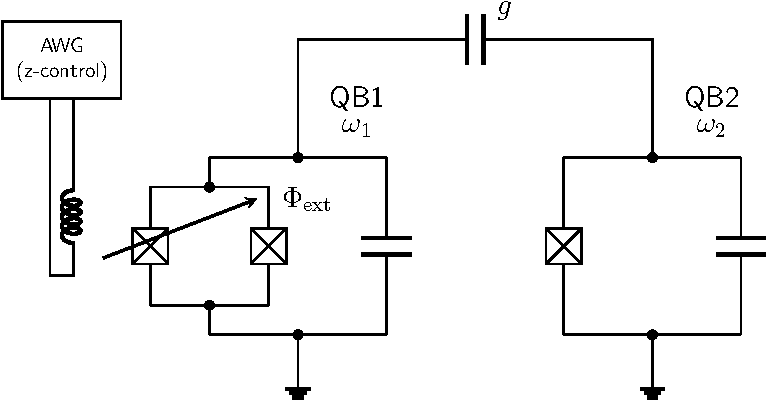
\includegraphics[width=0.8\textwidth]{fig/fig_z-ctrl.pdf}
  \caption{Target qubit architecture in our work. A tunable-frequency QB1 and a fixed-frequency QB2 are capacitively
    coupled with factor $g$.}
  \label{fig:z-ctrl}
\end{figure}
In superconducting quantum architectures, the ability to dynamically tune the transition frequency of a qubit is
essential for realizing the adiabatic $CZ$ gate.
This tunability is achieved by replacing the single Josephson junction of a standard
transmon with a superconducting quantum interference device (SQUID) loop as depicted in \fref{fig:z-ctrl},
which is then threaded by a localized magnetic
flux $\Phi_\text{ext}$ controlled via a dedicated microwave transmission line known as the $Z$-control line (or flux line).
% In \fref{fig:z-ctrl},
% \begin{equation}
%   % \begin{align}
%   \omega_1(\Phi_{\text{ext}})   = \frac{1}{\hbar} \left( \sqrt{8E_JE_C} \sqrt[4]{d^2 + (1 - d^2)
%       \cos^2(\pi \frac{\Phi_{\text{ext}}}{\Phi_0})} - E_C \right),
%   % \end{align}
%   \label{eq:flux}

\subsection{Qubit Architecture}
The system we consider is illustred in \fref{fig:z-ctrl}.
It is a system of two capacitively coupled transmon qubits, one fixed-frequency (QB2) and the other frequency tunable (QB1).
The simplified dispersive Jaynes-Cummings Hamiltonian for this system can be modeled as:
$$H = \sum_{i=1,2} \left( \omega_i \hat{a}_i^\dagger \hat{a}_i + \frac{\alpha_i}{2} \hat{a}_i^\dagger \hat{a}_i^\dagger \hat{a}_i \hat{a}_i \right) + g(\hat{a}_1^\dagger + \hat{a}_1)(\hat{a}_2^\dagger + \hat{a}_2) ,$$
where $g$ denotes the capacitive coupling strength between the two qubits, $\hat{a}_i^\dagger$ and $\hat{a}_i$ represent the
creation and annihilation operators for qubit $i$, respectively, and $\alpha_i$ defines the anharmonicity of qubit $i$.
Note that we use $\alpha$ for anharmonicity in discusion of the $CZ$ gates.
We use $\Delta$ and $\omega_i$ to denote different things. ($\Delta$ instead denotes the effective coupling strength
$2\sqrt{2}g$)
\subsection{Adiabatic Implementation}
CZ gate is a two-qubit gate that applies a phase flip to the target qubit if the control qubit resides in the state
$\ket{1}$. In the computational basis $\{\vert{}00\rangle, \vert{}01\rangle, \vert{}10\rangle, \vert{}11\rangle\}$, the
ideal unitary evolution is represented by a diagonal matrix:
\begin{equation}
  U_{\mathrm{CZ}}=\begin{pmatrix}
    1 & 0 & 0 & 0  \\
    0 & 1 & 0 & 0  \\
    0 & 0 & 1 & 0  \\
    0 & 0 & 0 & -1
  \end{pmatrix}.
\end{equation}
% The adiabatic CZ gate is realized as syncing the QB1's frequency to QB2's, thereby creating an avoided crossing.
% By doing so, the energy of $\ket{11}$ and $\ket{20}$ become comparable.
To implement this gate, the frequency of QB1 is swept along a
prescribed trajectory $\omega_1(t)$ toward the avoided crossing, held or continuously varied for a duration $\tau_d$,
and then returned to its idle parking frequency.
In this process, $\ket{11}$ obtains/loses more phases than the other computational states, due to its stronger coupling
to $\ket{02}$.

By following Refs.~\cite{Ding2025,Martinis2014}, we review the theory behind the adiabatic implementaion of the $CZ$ gate and
the derivation of the leakage formula \eref{eq:leakage}.
\begin{theorem}[Adiabatic Theorem]
  If a quantum system is initially prepared in a non-degenerate energy eigenstate of a time-dependent Hamiltonian, and
  if that Hamiltonian is varied sufficiently slowly, the system will evolve continuously to remain in the corresponding
  instantaneous eigenstate of the evolving Hamiltonian up to an accumulated phase factor, given that there is a gap
  between the eigenvalue and the rest of the Hamiltonian's spectrum.
\end{theorem}
Consider a two level system with the following Hamiltonian
$$
  H(t)=\eps(t)\sigma_z + \Delta\sigma_x.
$$
According to the adiabatic theorem, if we prepare the state $\ket{0}$ and slowly vary the Hamiltonian and then retrace the
change back, the resulting state is $\ket{0}$ with phase accumulation.
The instantaneous eigenstates are
\begin{equation}
  \vert{}\psi_-\rangle = \begin{bmatrix} -\sin(\theta(t)/2) \\ \cos(\theta(t)/2) \end{bmatrix} \quad \text{and} \quad \vert{}\psi_+\rangle = \begin{bmatrix} \cos(\theta(t)/2) \\ \sin(\theta(t)/2) \end{bmatrix},
\end{equation}
with eigenenergies
\begin{equation}
  E_- = -\frac{1}{2}\sqrt{\varepsilon(t)^2 + \Delta^2} \quad \text{and} \quad E_+ = \frac{1}{2}\sqrt{\varepsilon(t)^2 + \Delta^2},
\end{equation}
where
\begin{equation}
  \theta(t) = \arctan\frac{\Delta}{\eps(t)}.
  \label{eq:theta}
\end{equation}
We denote the energy difference of these two instantaneous eigenstates as
\begin{equation}
  \omega(t) = \sqrt{\varepsilon(t)^2 + \Delta^2}.
  \label{eq:omega}
\end{equation}

\subsubsection{Calculation of Leakage Error} \label{subsec:leakage}
Consider a state
$$
  \ket{\psi} = \alpha \ket{\psi_{-}}+\beta\ket{\psi_+} = \alpha_0\ket{0}+\beta_0\ket{1}
$$
with rotational change of coefficients
\begin{align*}
  \alpha & = \alpha_0\cos\dfrac{\theta}{2} + \beta_0\sin\dfrac{\theta}{2},  \\
  \beta  & =  \beta_0\cos\dfrac{\theta}{2} - \alpha_0\sin\dfrac{\theta}{2}.
\end{align*}
Differentiating with respect to time, we obtain
\begin{align*}
  \dot{\alpha} & = \dfrac{-i\omega \alpha+\beta \dot{\theta}}{2}, \\
  \dot{\beta}  & = \dfrac{i\omega \beta-\alpha \dot{\theta}}{2}.  \\
\end{align*}
By expressing the coefficients in terms of the angles $\alpha = \cos (\Theta/2)$ and $\beta=e^{i\phi}\sin(\Theta/2)$, we can
define
$$
  \alpha^* \beta = \dfrac{\sin\Theta e^{i\phi}}{2}.
$$
Calculating the time derivative of this quantity yields
$$
  \frac{d}{dt}(\sin\Theta e^{i\phi}) = i\omega \sin\Theta e^{i\phi}  \pm  \dot{\theta}\cos\Theta.
$$
Plugging $\phi=\phi_{\text{initial}} + \int_0^t\,\omega(t^\prime)\,\dd t^\prime$ and
symplifying the expression gives the approximate leakage probability $P_e=|\sin(\Theta(T)/2)|^2$,
\begin{equation}
  % \frac{d}{dt}(\sin\Theta e^{i\phi}) = i\omega \sin\Theta e^{i\phi}  \pm  \dot{\theta}\cos\Theta
  P_e \approx \dfrac{1}{4}\, \left\lvert\, \int_0^T \,\dfrac{\dd\theta}{\dd t} e^{-i\int\omega(t^\prime)\,\dd t^\prime}\right\rvert^2,
  \label{eq:leakage}
\end{equation}
with $T$ being a gate duration.
% If we assume that the time derivative of $\ket{\psi_-}$ and $\ket{\psi_+}$ are small enough, $\ket{\psi}$ evolves accordingly to \begin{align*}
%   \dot{\alpha} & = -iE_- \alpha, \\
%   \dot{\beta}  & = -iE_+\beta,
% \end{align*}
% in other words,
% \begin{align*}
%   \dot{\alpha} & = \dot{\alpha_0}\cos\dfrac{\theta}{2} + \dot{\beta_0}\sin\dfrac{\theta}{2},  \\
%   \dot{\beta}  & =  \dot{\beta_0}\cos\dfrac{\theta}{2} - \dot{\alpha_0}\sin\dfrac{\theta}{2},
% \end{align*}


\subsubsection{Dynamical and Conditional Phase Accumulation}
% According to the adiabatic theorem, if the sweep rate is sufficiently slow compared to the energy gap at the avoided crossing,
% the system will remain in its instantaneous eigenstate. The dynamic frequency excursion imparts a continuous deformation
% on the $\vert{}11\rangle$ state, causing it to hybridize temporarily with $\vert{}02\rangle$ and acquire a dynamical phase.
% The total accumulated phase $\Phi_{11}$ on the $\vert{}11\rangle$ state is the time integral of its instantaneous eigenenergy
% $E_{11}(t)$:$$\Phi_{11} = -\frac{1}{\hbar} \int_{0}^{\tau} E_{11}(t) dt$$
% Alongside the avoided crossing, the other states than $\ket{11}$ also acquire dynamical phases.
% To find the net phase $\ket{11}$ accumulates, we need to subtract these phases.
% % Simultaneously, single-qubit dynamical phases $\Phi_{01}$ and $\Phi_{10}$ are acquired.
% The conditional phase $\phi_{\text{cond}}$ accumulated over the gate duration is calculated
% by isolating the two-qubit interaction phase from the single-qubit contributions:
% $$\phi_{\text{cond}} = \Phi_{11} - \Phi_{01} - \Phi_{10} + \Phi_{00}$$
% The gate is successful when the pulse amplitude and duration are calibrated such
% that $\phi_{\text{cond}} = \pi \pmod{2\pi}$.
During the sweep towards the avoided crossing, computational states other than $\vert{}11\rangle$ also accumulate
dynamical phases. To determine the net phase acquired by the $\vert{}11\rangle$ state, these single-qubit contributions
must be subtracted. Specifically, the conditional phase $\phi_{\text{cond}}$ accumulated over the gate duration is
calculated by isolating the two-qubit interaction phase from the single-qubit contributions,
$$\phi_{\text{cond}} = \Phi_{11} - \Phi_{01} - \Phi_{10} + \Phi_{00},$$
where $\Phi_{ij}$ denotes phase accumulation for the state $\ket{ij}$.
A successful gate operation requires calibrating the pulse amplitude and
duration such that $\phi_{\text{cond}} = \pi \pmod{2\pi}$.

\subsubsection{Nonlinear time transformation}
By applying a time transformation, we can simplify the leakage formula \eref{eq:leakage}.
Let the time variable of this new frame be $\tau$. Set
$$
  \Delta \dd \tau = \omega(t) \dd t,
$$
then
\begin{equation}
  \dd t = \dfrac{\Delta}{\omega(t)}\dd \tau = \sin \theta(t) \dd \tau.
  \label{eq:nonlinear_time_transform_differential}
\end{equation}
In integral form,
\begin{equation}
  t(\tau) = \int_0^\tau\,\sin\tilde{\theta}(\tau^\prime)\,\dd\tau^\prime.
  \label{eq:nonliniear_time_transform}
\end{equation}
The virtue of this transformation is clear if we plug \eref{eq:nonlinear_time_transform_differential} into \eref{eq:leakage},
\begin{equation}
  P_e = \dfrac{1}{4}\, \left\lvert\, \int_0^\tau\,\dfrac{\dd\tilde{\theta}}{\dd\tau}\, e^{-i\Delta \tau}\,\dd \tau \right\rvert^2.
  \label{eq:leakage_tau}
\end{equation}
The leakage error is expressed as the Fourier transform of $\dfrac{\dd\tilde{\theta}}{\dd \tau}$
at $\Delta$.


\subsection{Slepian pulses}

% In the context of pulse waveform optimization, the Slepian pulses, frequently referred to as discrete prolate spheroidal
% sequences (DPSSs), represent a family of orthogonal pulses specifically formulated to solve the problem of maximal
% energy concentration in both the time and frequency domains. Because Heisenberg's uncertainty principle dictates that a
% pulse cannot be strictly bounded in both time and frequency simultaneously, Slepian, Landau, and Pollack developed these
% sequences to answer a fundamental optimization question: how to optimally concentrate energy in one domain when the
% pulse is strictly confined in the opposing domain.

A (discrete) Slepian pulse is a finite-length discrete time signal which maximazes the energy concentration in a prescribed
frequency band $[-W,W]$.
The exact formula for this pulse can be derive by considering the following eigenvalue problem.

Consider a discrete-time pulse of finite length, denoted as $x[n]$ for $n = 0, 1, \dots, N-1$.
Its energy concentration in $[-W,W]$ is
\begin{equation}
  \frac{\int_{-W}^{W} \vert{}X(e^{i\omega})\vert{}^2 d\omega}{\int_{-\pi}^{\pi} \vert{}X(e^{i\omega})\vert{}^2
    d\omega},
  \label{eq:energy_concentration}
\end{equation}
where $X$ denotes discrete Fourier transform,
$$X(e^{i\omega}) = \sum_{n=0}^{N-1} x[n]e^{-i\omega n}.$$
The \eref{eq:energy_concentration} can be rewritten as
$$\dfrac{x^TAx}{x^Tx}$$
where $x$ is the vector form of the signal $x[n]$ and $A$ is a matrix with $A_{n,m} = \frac{\sin 2\pi W(n - m)}{\pi(n - m)}$.

$A$ has $N$ eigenvalue solutions and the eigenvector corresponding to the second largest eigenvalue satisfies
anti-symmetric property $x[n] = -x[N-1-n]$.

\subsection{Limitations of Slepian Pulses}
While the Slepian pulse is widely utilized and exhibits an excellent spectral profile with exceptionally low sidelobes,
it is not strictly optimal for this specific application.
As demonstrated in \eref{eq:leakage_tau}, the leakage error depends exclusively on the Fourier transform evaluated at the precise
frequency $\Delta$. Consequently, this leaves significant room for further targeted waveform optimization.
    % Background
\section{Methods}
\label{sec:proposed}
In this section, we investigate methods to mitigate leakage errors in X and CZ gates, beginning with the X gate. Our
approach builds on the DRAG-1 scheme. Conventionally, DRAG-1 relies on a seed function to generate a control pulse to
minimizes leakage from $\vert{}0\rangle$ to $\vert{}2\rangle$. However, we demonstrate that bypassing the seed function
to synthesize the pulse directly yields a superior pulse shape.
% \subsection{X gate}
\subsection{Note on $Y$ DRAG correction}
Aside from the $X$ control pulse, we utilize the DRAG pulses \ref{eq:ydrag} and \ref{eq:zdrag}.
We demonstrate that the analytical expression for the $Y$ control pulse remains valid even in the non-perturbative
regime---a derivation that, to the best of our knowledge, has not been previously reported in the literature. To
illustrate this, we recalculate the system Hamiltonian without relying on perturbative assumptions. We introduce a
unitary frame transformation $V$, defined as:
% We can show that the formula for the $Y$ control pulse is still valid in non-perturbative regime.
% (Within the knowledge of the author, this computation has not been done/shown elsewhere.)
% Now we recalculate the Hamiltonian without the assumption of perturbation.
% % Applying a frame change with $V=\exp(S)$, $S=-i\lambda_2\dfrac{\Omegax}{2\Delta_2}\hat{\sigma}^y_{1,2}$ to the Hamiltonian \ref{eq:Hrwa} ,
% % the new $\ket{1}\bra{2}$ component reads
% Consider a frame change $V$
\begin{equation}
  V = \exp\left[-i\lambda_2\dfrac{\Omegax}{2\Delta_2}\hat{\sigma}^y_{1,2}\right]
  = \cos(\phi) -i\hat{\sigma}^y_{1,2}\sin(\phi)
  \label{eq:first_frame_change}
\end{equation}
where $\phi = \lambda_2\dfrac{\Omegax}{2\Delta_2}$, and apply it to our qudit Hamiltonian in \eref{eq:Hrwa}.
The $\ket{1}\bra{2}$ component of the resulting Hamiltonian is
$$
  -\sin(2\phi)\dfrac{\delta(t)+\Delta}{2}+\cos(2\phi)\dfrac{\lambda \Omegax}{2}-i\dfrac{\lambda}{2}\left(\dfrac{\Omega_x^\prime(t)}{\Delta}+\Omega_y(t)\right).
$$
% Setting $\Omegay$ as in \eref{eq:ydrag} still reduces this component.
% Hence, we just use the standard DRAG correction \eref{eq:ydrag} for the $Y$ control.
Substituting $\Omega_y$ as defined in \eref{eq:ydrag} demonstrates that this off-diagonal component is still effectively
suppressed. Consequently, we retain the standard DRAG correction  for the $Y$ control pulse.
% \subsection{RWA}



% \subsubsection{Antidiagonalization of $2\times 2$ matrix}
%
% \begin{boxA}
%   {\bf Probelm } \\
%   Given a Hermitian matrix $H\in M_2(\CC)$, antidiagonalize $H$ so that its diagonal elements be minimized according to transformation~(\ref{eq:framechange}).
% \end{boxA}
% Suppose $H$ is a $2\times2$ Hermitian matrix.
% Consider a problem of anti-diagonlizing $H$ according to the transformation~\ref{eq:framechange}.
% Here we mean by anti-diagonalization making the diagonal components as small as possible in the sense of $l_1$ or $l_2$ sum.
%
% $$
%   H    = H_d + H_a, \qquad
%   H_d  = \begin{pmatrix} a(t) & 0 \\ 0 & d(t) \end{pmatrix},\qquad
%   H_a  = \begin{pmatrix} a(t) & 0 \\ 0 & d(t) \end{pmatrix}
% $$
% Consider the following transformation:
% \begin{equation}
%   U(t) = \exp\left(i\int_0^t\,H_d(t^\prime)\mathrm{d}t^\prime\right) = \begin{pmatrix}\exp\left(i\int_0^t\,a(t^\prime)\mathrm{d}t^\prime\right) &0\\0&\exp\left(i\int_0^t\,d(t^\prime)\mathrm{d}t^\prime\right) \end{pmatrix}
%   \label{eq:antidiagonalization}
% \end{equation}
% Since $i\dot{U}U^\dagger=-H_d(t)$, this yields a complete anti-diagonalization
% $$
%   H^\prime(t) =
%   \begin{pmatrix}
%     0                 & b(t)e^{i\phi(t)} \\
%     c(t)e^{-i\phi(t)} & 0                \\
%   \end{pmatrix}
% $$
% where $\phi(t) = \int_0^t\,[a(\tau)-d(\tau)]\mathrm{d}\tau$.
%
% To make this method effective, we need to ensure that $\ket{0}$ and $\ket{1}$ has not changed at the ends of the
% operation by the transformation~\ref{eq:antidiagonalization}. In formula,
% $$
%   \phi(T) \in \RR_{>0}
% $$

\subsection{DRAG-1}
Although in \ref{subsec:drag}, the DRAG-1 pulse is created from the seed pulse waveform $\Omega_1$
through \eref{eq:drag1}, now we reverse this process.
First we solve \eref{eq:drag1} for $\Omega_1(t)$.
We can rewrite  \eref{eq:drag1} as a second-order linear oridnary differential equation (ODE):
\begin{equation}
  \Omega^2_x(t)=\left(1+\frac{D^2}{\Delta_2^2}\right)\Omega_1^2(t).
  \label{eq:drag1_ode}
\end{equation}
Recognizing this as a driven harmonic oscillator equation, the general solution is
\begin{equation}
  \Omega_1^2(t) = \int_0^t\,\left[\dfrac{1}{\Delta_2}\sin(\Delta_2(t-\tau))\right][\Delta_2^2\Omega_x(\tau)^2]\,\dd \tau
  + A\cos(\Delta_2t+\phi).
  \label{eq:drag1_sol}
\end{equation}
The first term represents the particular solution to the ODE in \eref{eq:drag1_ode}.
The verification can be done with
the Leibniz rule \cite{apostol}, which governs the differentiation under the integral sign:
\begin{equation}
  \frac{d}{dt} \int_{a(t)}^{b(t)} F(x,t) dx = F(b(t), t) \cdot b'(t) - F(a(t), t) \cdot a'(t) + \int_{a(t)}^{b(t)} \frac{\partial}{\partial t} F(x,t) dx.
  \label{eq:leibniz}
\end{equation}
Recall we have three boundary conditions on our debt:
\begin{enumerate}
  \item $\Omega_x = 0$ at both ends ($t=0$, $T$): This ensures compatibility with the SWT and enforces boundary continuity for the X-pulse, mitigating spectral leakage.
  \item $\dot{\Omega}_x = 0$ at both ends ($t=0$, $T$): This guarantees a smooth envelope derivative, maintaining essential boundary continuity for the corresponding Y-pulse.
  \item $\Omega_1 = 0$ at both ends ($t=0$, $T$): This further enforces strict SWT compatibility at the start and completion of the gate.
\end{enumerate}

Applying the third boundary condition at the initial time $t = 0$  immediately eliminates the homogeneous component, yielding $A = 0$ in \eref{eq:drag1_sol}
The constraint at $t=T$ translates to
$$
  \left(\Omega_1^2(T)\right) = 0 = \int_0^T\,\left[\dfrac{1}{\Delta_2}\sin(\Delta_2(T-\tau))\right][\Delta_2^2\Omega_x(\tau)^2]\,\dd \tau,
$$
differentiating both sides we get
$$
  \left(\Omega_1(T)\dot{\Omega}_1(T)\right) = 0 = \int_0^T\,\left[\cos(\Delta_2(T-\tau))\right][\Delta_2^2\Omega_x(\tau)^2]\,\dd \tau.
$$
These two constraints combined implies
$$
  \int_{-\infty}^{\infty}[\Delta_2^2\Omega_x(\tau)^2]e^{-i\Delta\tau}\,\dd \tau.
$$
Hence, The boundary condition at $t=T$ for smoothness translates to the null fourier transform condition,
\begin{equation}
  \int_0^T \Omega_x(\tau)^2 e^{-i\Delta_2\tau} d\tau = 0.
  \label{eq:drag1_fourier}
\end{equation}
\subsubsection{Pulse Design}
Although Jesus et al. \cite{99999} proposed a pulse design method for $\Omega_x$ by way of $\Omega_1$, and investigated
an optimal pulse waveform therein, we can
directly design a DRAG-1 pulse through \eref{eq:drag1_fourier}.
Now we consider pushing the gate time limit for maintaining the perturbative approximation of Schrieffer-Wolff transformation.
In it,
The problem of early truncation will be somewhat relieved by keeping $\max |\Omega_x|$ small.
We combine delayed leakage reduction technique described in \cite{Polat2026} and function design techniques to obtain
such pulses.

Let $t_d=\pi/\Delta$. Then $f(t)+f(t-t_d)$'s Fourier transform is computed as
$$
  \mathcal{F}[f(t)+f(t-t_d)](\Delta) = \mathcal{F}[f](\Delta)+e^{i\Delta t_d}\mathcal{F}[f](\Delta) = 0.
$$
This suggests that we find a function $g(t)$ on $[-1,1]$ that satisfies the following property:
\begin{enumerate}
  \item \label{itm:g1} $g$ is anti-symmetric
  \item \label{itm:g2} $g$ is monotonically increasing
  \item \label{itm:g3} $g(1)=1/2$
  \item  \label{itm:g4} $g$'s first and second derivative vanishes at $g(-1)$.
\end{enumerate}
$g$ represents the function on $[0,t_r]$.
On obtaining such a $g$, we construct $\Omega_x^2$ as
$$
  \Omega_x^2(t) =
  \begin{cases}
    A \left(g(2t/t_r-1)-g(-1)\right) \quad                     & (0<t<t_r)       \\
    A                         \quad                            & (t_r<t<t_d)     \\
    A\left( g(2(t_r+t_d-t)/t_r-1)-g(-1)\right)           \quad & (t_d<t<t_d+t_r) \\
  \end{cases}
$$
where $A$ is the amplitude determined by integrating $\Omega_x^2$ according to \eref{eq:xgate_condition}.

There are mutliple choices for such $g$.
\begin{enumerate}
  \item $\dfrac{1}{2} x+\dfrac{1}{2\pi}\sin( \pi x)$
  \item $3\pi x+4\sin(\pi x)+\dfrac{1}{2} \sin(2\pi x)$
\end{enumerate}
\subsubsection{$g$ design}
Let $h$ be a positive symmetric function on $[-1,1]$ that vanishes at both ends.
Put $g^\prime = h^2$. This ensures that the condition \ref{itm:g4} holds as $g^{\prime\prime}=2hh^\prime=0$
and it is easy to check that the other condtions \ref{itm:g1}-\ref{itm:g3} are also satisfied.

\subsection{Optimization by Riccati engineering}
As we've seen in \ref{subsec:npad}, NPAD has an obvious issue that the Hamiltonian is assumed to be
time-independent, and in Ref.~\cite{NPAD2022}, the author only applies this method to perturbative cases, in which the
method reduces to recursive Schrieffer-Wolff transformations.

We outline the newly proposed procedure to handle non-perturbative cases.
% Although well known as a qunatum control method, Ricatti engineering is not widely applied to one qubit gate control.
% In this subsection, we see how Riccati engineering described in \cite{Riccati2010} reduces to in the case of
% dimension $3$.
% Given a $3\times 3$ matrix $H$, we consider the problem of block diagonalizing it into $2\times 2$ and $1\times 1$
% compartments.
% Write
% $$H(t) = \begin{pmatrix} H_11(t) & H_{12}(t) \\ H_{21}(t) & H_{22}(t) \end{pmatrix}$$
% $H'(t) = U(t)H(t)U^\dagger(t) + i\dot{U}(t)U^\dagger(t)$.
% $$U(t) = \begin{pmatrix} (I_2 + X^\dagger X)^{-1/2} & X^\dagger (I_{n-2} + X X^\dagger)^{-1/2} \\ -X (I_2 + X^\dagger X)^{-1/2} & (I_{n-2} + X X^\dagger)^{-1/2} \end{pmatrix}$$
% where $X(t)=(x_1(t)\:\:\: x_2(t))$
% \begin{equation}
%   i\dot{X} = H_{21} + H_{22}X - XH_{11} - XH_{12}X \label{eq:riccati}
% \end{equation}
% First we see how the results in \ref{subsec:ricatti} apply to the Hamiltonian
Applying to the qudit Hamiltonian \ref{eq:rotatingframe} with $N_{\rm{max}}=2$,
the Riccati equation becomes
$$i\dot{x}_1 = (2\delta+\Delta) x_1 - \frac{1}{2}(\Omega_x + i\Omega_y)x_2 - \frac{\lambda}{2}(\Omega_x - i\Omega_y)x_1 x_2,$$
$$i\dot{x}_2 = \frac{\lambda}{2}(\Omega_x + i\Omega_y) + (2\delta+\Delta) x_2 - \frac{1}{2}(\Omega_x - i\Omega_y)x_1 - \frac{\lambda}{2}(\Omega_x - i\Omega_y)x_2^2.$$
If we define
\begin{equation}
  A = -\frac{1}{2}(x_2^2+\lambda x_1)\label{eq:A}
\end{equation}
\begin{equation}
  B = \frac{1}{2}x_1^2 \label{eq:B}
\end{equation}
\begin{equation}
  C = i(\dot{x_1}x_2-x_1\dot{x_2}) \label{eq:C}
\end{equation}
Then $\Omega_x$, $\Omega_y$, and $\delta(t)$ can be expressed
\begin{equation}
  \tilde{\Omega} = \Omega_x+i\Omega_y = \dfrac{A^\star C - B C^\star}{|A|^2-|B|^2}, \label{eq:riccati_Omega}
\end{equation}

\begin{equation}
  \delta(t) = \frac{1}{2} \left( \frac{i\dot{x}_1 + \frac{1}{2} x_2 \tilde{\Omega} + \frac{1}{2}\lambda x_1 x_2 \tilde{\Omega}^*}{x_1} - \Delta_2 \right) \label{eq:riccati_delta}.
\end{equation}



\subsubsection{Variational method}
One way to utilize \eref{eq:riccati_Omega} and \eref{eq:riccati_delta} is to determine $x_1$ and $x_2$ first and
solve numerically for $\tilde{\Omega}$ and $\delta$.
There's multiple difficulties with this approach. Since the Riccati equation \eref{riccati} is not linear, adjust the
pulse area of $\Omega_x$ is difficult. To overcome this issue, we first derive the and then
In this study, Riccati engineering method is utilized as an optimization method,
To preserve the X gate condition \eref{eq:xgate},
\begin{equation}
  \delta \Theta = \int_0^T \sum_{k=1}^2 \left( \frac{\partial \Omega_x}{\partial x_k} \delta x_k + \frac{\partial \Omega_x}{\partial \dot{x}_k} \delta \dot{x}_k + \text{c.c.} \right) dt
\end{equation}
must vanish. ($\dfrac{\partial}{\partial x_i}$ denotes Wirtinger derivatives.)
Integral by parts transforms the above equation into

\begin{equation}
  \delta \Theta = \left[ \sum_{k=1}^2 \left( P_k(T) \delta x_k(T) + P_k^*(T) \delta x_k^*(T) \right) \right] + \int_0^T \sum_{k=1}^2 \left( G_k(t) \delta x_k(t) + G_k^*(t) \delta x_k^*(t) \right) dt.
\end{equation}
Note that $\delta x_k(0) = 0$.


$$G_k(t) = \frac{\partial \Omega_x}{\partial x_k} - \frac{d}{dt} \left( \frac{\partial \Omega_x}{\partial \dot{x}_k} \right)$$

$$P_1(t) = \frac{\partial \Omega_x}{\partial \dot{x}_1} = i \frac{A^* - B^*}{2(\vert{}A\vert{}^2 - \vert{}B\vert{}^2)} x_2$$

$$P_2(t) = \frac{\partial \Omega_x}{\partial \dot{x}_2} = -i \frac{A^* - B^*}{2(\vert{}A\vert{}^2 - \vert{}B\vert{}^2)} x_1$$


\subsection{CZ gate}
In this section, for brevity, the length of pulses are assumed to be $N$, an odd number.
As seen in \ref{subsec:leakage}, the leakage error is approximately expressed as $\dfrac{1}{4}|G(\Delta)|^2$.
In the following we propose several methods to mitigate this error.
\subsubsection{anti-symmetric Chebyshev pulse}
Maintaining a specified sidelobe level, Chebyshev pulse is the signal that minimizes the mainlobe width

Mathematically, a chebyshev pulse $g_{ch}$ is a discrete time pulse defined as
$$
  g_{\text{ch}}[n] = \frac{1}{N} \Bigg[ 1 + 2r \sum_{k=0}^{(N-1)/2} (-1)^k T_{N-1}\left(x_0 \cos \frac{\pi k}{N}\right)  \cos \left( \frac{2\pi k}{L} \left(n + \frac{1}{2}\right) \right) \Bigg], $$
where $r = \frac{1}{T_{N-1}(x_0)}$ corresponds to the suppressed sidelobe level.
We call its anti-symmetrization
$$
  g_{ach}[n] = \begin{cases}
    g_{ch}[n]  \quad     & n< (N+1)/2  \\
    0             \quad  & n = (N+1)/2 \\
    -g_{ch}[N-n]   \quad & n > (N+1)/2 \\
  \end{cases}
$$
anti-symmetric Chebyshev pulse $g_{ach}$.
\subsubsection{Correctional Derivative pulse}
To reduce the fourier transform at $\Delta$, recall that
$$
  \mathcal{F}[f^\prime](\Delta) = i\omega \mathcal{F}[f](\Delta).
$$
Hence, by adding the second derivative to $f$, we can reduce the fourier transform to $0$,
$$
  \mathcal{F}[(1+D^2/\Delta^2)f](\Delta) = 0.
$$
This method is only applicable to pulses whose second derivative is anyti-symmetric, such as anti-symmetric Chebyshev,
to maintain the anti-symmetric property after adding the second derivative.


\subsubsection{Combining two pulses}
Combining two pulses of different origins
\subsubsection{Redefining the Slepian eigenvalue problem}
The (second) Slepian pulse is the solution of the second largest eigenvalue to the following problem
\begin{equation}
  \dfrac{\int_{-W}^{W}\,|G_{\text{DTFT}}(\omega)|^2 d\omega}
  {\int_{-\pi}^{\pi}\,|G_{\text{DTFT}}(\omega)|^2 d\omega} = \dfrac{g^TA_{m,n}g}{g^Tg} \label{eq:slepproblem}
\end{equation}
where $A_{m,n} = \sinc(\pi(m-n)W) = \dfrac{\sin(\pi(m-n)W)}{\pi(m-n)W}$.
(\ref{eq:slepproblem}) is the eigenvalue problem of the matrix $A_{m,n}$. It was Slepian who found a commuting
matrix for $A_{m,n}$ and solev teh problem analyitcally.

Close investigation of the \eref{eq:leakageerror}



For the targetted range of $W_1\leq \dfrac{T}{N}  \Delta \leq W_2$
$$\text{minimize } \frac{\int_{W_1}^{W_2} \vert{}G_{\text{DTFT}}(\omega)\vert{}^2 d\omega}{\int_{W_1}^{W_2} \vert{}G_{\text{DTFT}}(\omega)\vert{}^2 d\omega} = \frac{\tilde{g}^T (A_{\text{rect}}(W_2) - A_{\text{rect}}(W_1)) \tilde{g}}{\tilde{g}[0]^2 + \dots + \tilde{g}[N]^2}$$
To not elongate gate time we impose the following condition,
$\tilde{g}$ should be anti-symmetric and non-negative on the first half.
\begin{itemize}
  \item $\tilde{g}[s] = \tilde{g}[N-1-s]$
  \item $\tilde{g}[s] \geq 0 \quad \text{for }0\leq s\leq L-1$
\end{itemize}
Put
$$B = \begin{pmatrix} 1 & & \\ & \ddots & \\  &  & 1\\0 & \cdots & 0 \\  &  & -1 \\& \mathinner{\mkern2mu\raise1pt\hbox{.}\mkern2mu\raise4pt\hbox{.}\mkern2mu\raise7pt\hbox{.}\mkern1mu} & \\ -1 & &  \end{pmatrix}, \quad C = B^T A B$$
$$\begin{pmatrix} \tilde{g}[0] \\ \vdots \\ \tilde{g}[N] \end{pmatrix} = B \begin{pmatrix} h[0] \\ \vdots \\ h[L-1] \end{pmatrix}$$
Then
$$\text{maximize } -\frac{h^T C h}{h^T h}$$
is the problem to solve.
\subsubsection{Sequential Quadratic Programming}
Given an ansatz and an evaluation point $\Delta$, the algorithm goes as follows:

\begin{algorithm}
  \caption{Variational Quantum Circuit Optimization}\label{alg:vqa_opt}
  \begin{algorithmic}[1] % The [1] enables line numbering
    \Require Target unitary $U$, Error tolerance $\epsilon$
    \Ensure Optimized parameters $\boldsymbol{\theta}$
    \State Initialize $\boldsymbol{\theta} \gets \text{random values in } [0, 2\pi]$
    \State Set learning rate $\alpha \gets 0.01$
    \While{cost function $\mathcal{L}(\boldsymbol{\theta}) > \epsilon$}
    \State Compute gradient $\nabla \mathcal{L}(\boldsymbol{\theta})$ using parameter-shift rule
    \If{$\|\nabla \mathcal{L}(\boldsymbol{\theta})\| < \text{threshold}$}
    \State \textbf{break} \Comment{Early stopping criteria}
    \EndIf
    \State $\boldsymbol{\theta} \gets \boldsymbol{\theta} - \alpha \nabla \mathcal{L}(\boldsymbol{\theta})$
    \EndWhile
    \State \Return $\boldsymbol{\theta}$
  \end{algorithmic}
\end{algorithm}

    % Background
\section{Simulation and Numerical Results}
\label{sec:result}
For quantum simulation, we used QuTiP5 \cite{qutip5} software.
We first see the results from $X$ gate simulation.
\subsection{X gate}
Simulation has been conducted with the Hamiltonian in \eref{eq:Hrwa} with $N_{max}=3$.
Among several solvers that QuTiP provides, the Shroedinger solver has been chosen.
This is enough unless your target fidelity level is exceedingly low so that the effect of decoherence is visible in the
duration of one gate operation.
The parameters we use for this simulation are
\begin{itemize}
  \item $\Delta/2\pi = -0.225~\text{GHz}$ (anharmonicity),
  \item $\lambda_k = \sqrt{k}$.
\end{itemize}
We set the time slice number of the ODE solver as $25000$. (Increasing this number didn't change the simulation results.)
% We chose the proportionality constant of $\lambda_{k,k+3}$ as $c=0.004$ , we set
% $\lambda_k = \sqrt{k}$, $\lambda_{k,k+3}=c\sqrt{k+1}\sqrt{k+2}\sqrt{k+3}$, with .
% The $X$ gate was implemented with different pulse shapes.
\subsubsection{Fidelity}
The gate infidelity was computed as $\mathcal{E}(\hat{U}_Q) = 1 -
  \mathcal{F}[\hat{U}_Q]$ where $\mathcal{F}[\hat{U}_Q]$ is the gate fidelity defined as
\cite{fidelity}
\begin{equation}
  \label{eq:fidelity}
  \mathcal{F}[\hat{U}_Q] = \frac{\text{Tr}[\hat{U}_Q\hat{U}_Q^\dagger]}{d(d+1)} +
  \frac{\left\vert{}\text{Tr}[\hat{U}_Q\hat{U}_I^\dagger]\right\vert{}^2}{d(d+1)}.
\end{equation}

\begin{figure}[htpb]
  \centering
  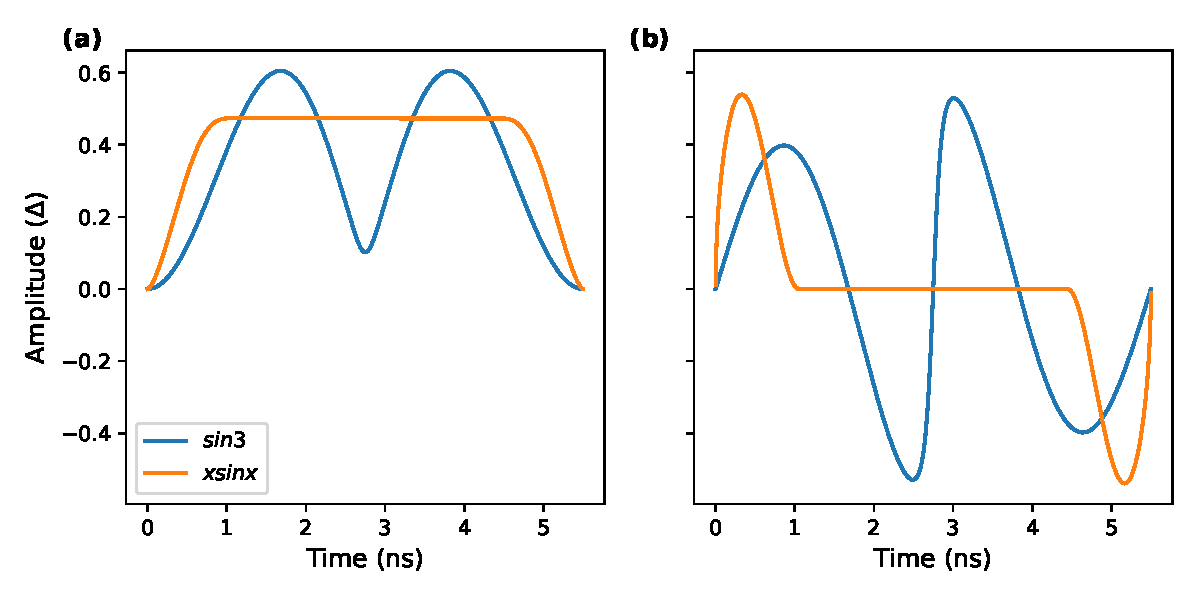
\includegraphics[width=0.8\columnwidth]{fig/fig_r1d_comparison.pdf}
  \label{fig:r1d_comparison}
  \caption{Comparison of $X$ and $Y$ controls of our DRAG-1 (orange) and R1D (blue) pulses.
    (a) $X$ control, (b) $Y$ control.
  }
\end{figure}


\begin{figure}[htpb]
  \centering
  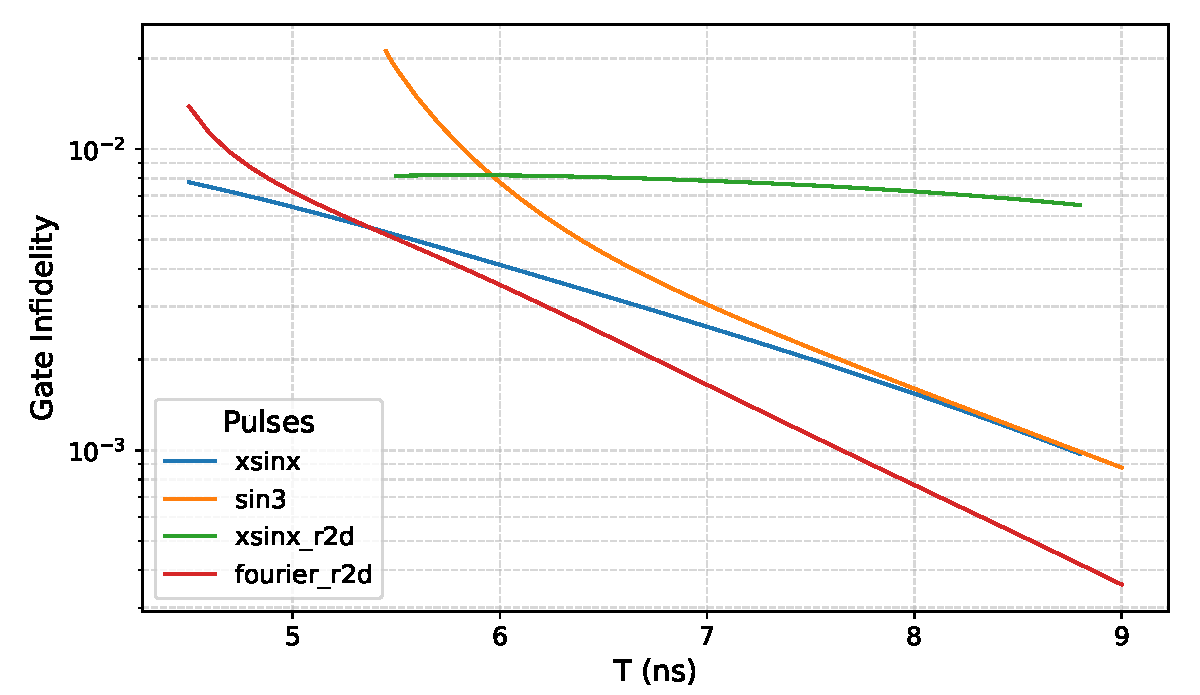
\includegraphics[width=0.8\columnwidth]{fig/fig_gateinfidelity.pdf}
  \label{fig:gate_infidelity}
  \caption{Although our DRAG-2 pulse shows poor performance,
    our DRAG-1 pulse surpasses the performance of the R2D pulse for $T< 5.3~\text{ns}$.}
\end{figure}

\begin{figure}[htpb]
  \centering
  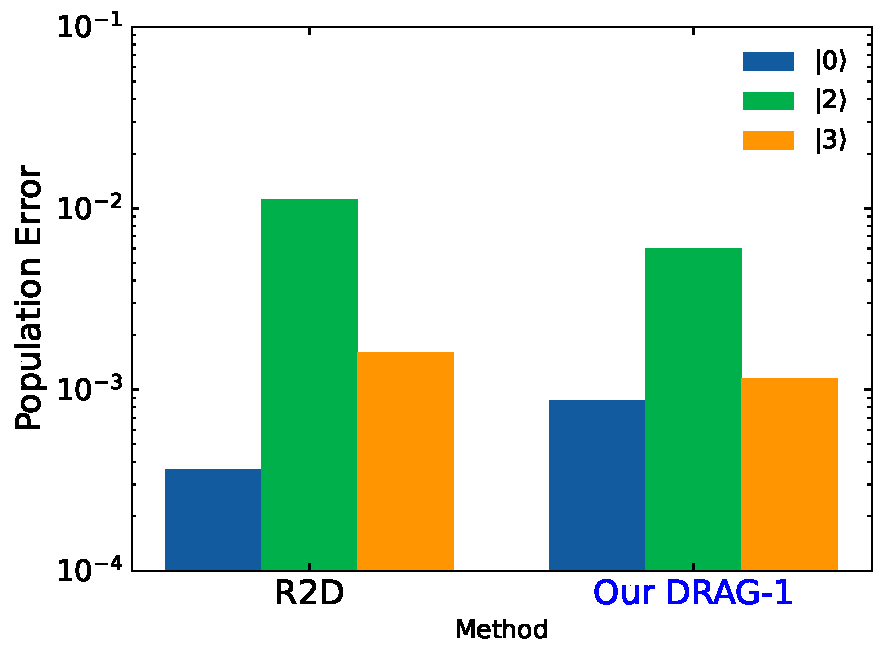
\includegraphics[width=0.8\columnwidth]{fig/fig1d.pdf}
  \label{fig:r2dvsxsinx}
  \caption{Population distirbution of $X$ gate for $T=4.8~\text{ns}$ implemented by R2D and our DRAG-1 pulse.
    The main error comes from the leakage to $\ket{2}$ in both cases.
    % If we numerically calculate $\Omega_1$ for our  DRAG-1 pulse,
    % there's a possibility of overtaking the best-performing R2D.
  }
\end{figure}
\subsubsection{Pulse shapes}
In our simulaiton setting, $t_d = 2.2~\text{ns}$.

\noindent\textbf{DRAG-1 Pulse}\\
For this analysis, two variations of DRAG-1 pulses were synthesized. The first was derived via the standard differential
method using the seed function $\sin^3(\pi t/T)$. The second was constructed using our proposed methodology, which is
characterized by a rising edge function of the form $g(t) = x + \sin(x)$. Throughout the remainder of this text, the
pulse based on the $\sin^3(\pi t/T)$ seed is designated as R1D, while the pulse generated by our novel approach is
referred to as our DRAG-1.
% We created two DRAG-1 pulses, one with the differential method with the seed function $\sin^3(\pi t/T)$, the other with
% our novel method with the rising edge $g(t)$ of form $g(t) = x+\sin(x)$. Henceforth we refer to $\sin^3(\pi t/T)$ as
% R1D, and the latter one as our DRAG-1.

\noindent\textbf{DRAG-2 Pulse}\\
In \cite{universalpulse}, the pulse shape
$$
  \dfrac{1}{16}\cos(6\pi )-\dfrac{9}{16}\cos(\pi\dfrac{2t}{t_f})+\dfrac{1}{2}.
$$
is a versatile initial pulse shape for recursive DRAG framework. We call R2D for the DRAG-2 pulse created from this pulse.

With the function $h(t)$ being a raised cosine function, we curated our DRAG-2 pulse.
The pulse shape for $T=5.5~\text{ns}$ is shown in \fref{fig:r2d_xy}.

% We applied DRAG corrections to all pulses.

\subsubsection{Performance}
In \fref{fig:gate_infidelity}, we compare the gate infidelity between these four pulses.
DRAG-1 outperformed and showed its effectiveness within short gate durations ($<5~\text{ns}$).
As the gate duration decreases, both R1D and R2D exhibit a non-linear degradation in performance. This is attributed to
the increased pulse amplitude, which compromises the accuracy of the SWT approximation. Compared to R1D and R2D, our
DRAG-1 is specifically designed to suppress this amplitude growth. Consequently, its gate infidelity-gate duration
characteristic remains consistent regardless of reductions in gate time.
% We compared four pulses xsinx, Hann, fourier
\subsubsection{Minimum Gate Time of Our DRAG-1}
Using the echo method in the construction of the DRAG-1 pulse, as in our proposed method, has
the minimum gate time limit
$$T=t_r+2t_d\geq 2t_d\approx4.44~\text{ns}.$$
The minimum gate time of the Hann-type pulse is known to be $\sqrt{6}t_d\approx5.44$ %in our simulation, the graph is plotted right up to this limit in \fref{fig:gate_infidelity}.).
Hence, our DRAG-1 pulse has reduced $20\%$ of gate duration compared to the R1D pulse.
% Further, in our simulation, we confirmed that our DRAG-1 pulse didn't degrade if we let the gate duration approach to this limit.

Conventional transmons anharmonicity ranges from $-150$ to $-300~\text{GHz}$ \cite{currentstateofplay}, corresponding to $t_d= 1.7~\text{ns}$ to $3.3~\text{ns}$.
Hence, the minimum gate duration of our method when applied to different transmon qubits ranges from $3.4~\text{ns}$ to
$6.6~\text{ns}$.

\subsubsection{Limitations on our proposed design of DRAG-2 Pulse from the Echo Method}
\begin{figure}[htpb]
  \centering
  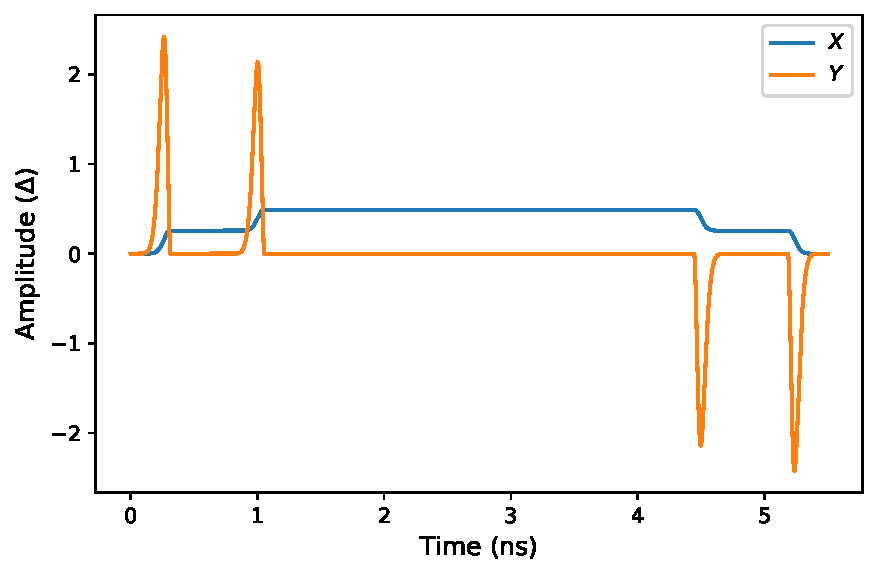
\includegraphics[width=0.8\columnwidth]{fig/fig_r2d_xy.pdf}
  \label{fig:r2d_xy}
  \caption{
    % Limitation of the proposed method for DRAG-2
    DRAG-2 pulse for $T=5.5~\text{ns}$.
    $t_r<\dfrac{2}{3}t_d$ degrades the gate performance and
    sharp edges arise in the $Y$ control.
  }
\end{figure}
In our proposed DRAG-2 design scheme,
using the echo method in the construction of the rising edge of $f(t)$ in \fref{fig:drag1} carries several difficulties.
First, it imposes us a minimum gate time limit as $ t_r>t_d/3 $,
$$
  T = 2t_d+t_r > 7/3t_d\quad\text{Our method.}
$$
If we could use a different method to construct $f(t)$ in \fref{fig:drag1}, this limit can be pushed to
$$
  T = 2t_d+t_r > 5/2t_d\quad\text{Theoretical limit.}
$$
The minimum gate duration degrades by $7\%$.
It has another problem of introducing edges into the $Y$ control pulse as illustrated in \fref{fig:r2d_xy}.
This is because if $t_r <2/3t_d$, $h(t)$ in \fref{fig:drag2} becomes short in duration.
Although designed as a DRAG-2 pulse, and inherently performs better than DRAG-1,
% \subsubsection{Simulation settings}
% \begin{figure}
%   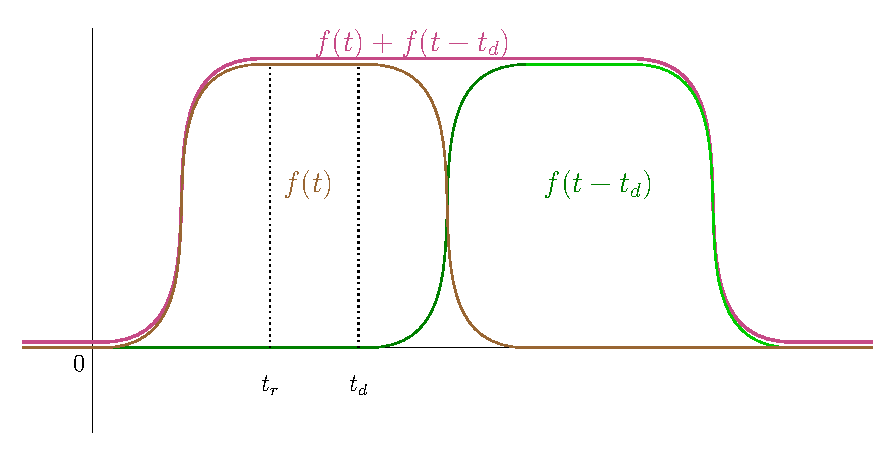
\includegraphics[scale=.3]{fig/fig_drag1.pdf}
% \end{figure}
% The
% is created with
% $ \Omega_1(t) = \Omega_0\sin^3(\pi t/T) $, which gives
% $$
%   \Omega(x) =
% $$
% The maximum value of which is

\subsubsection{Non-perturbative Validation of the $Y$-DRAG Correction}
Aside from the $X$ control pulse, we utilize the DRAG pulses \ref{eq:ydrag} and \ref{eq:zdrag}.
We demonstrate that the analytical expression for the $Y$ control pulse remains valid even in the non-perturbative
regime---a derivation that, to the best of our knowledge, has not been previously reported in the literature. To
illustrate this, we recalculate the system Hamiltonian without relying on perturbative assumptions. We introduce a
unitary frame transformation $V$, defined as:
\begin{equation}
  V = \exp\left[-i\lambda_2\dfrac{\Omegax}{2\Delta_2}\hat{\sigma}^y_{1,2}\right]
  = \cos(\phi) -i\hat{\sigma}^y_{1,2}\sin(\phi)
  \label{eq:first_frame_change}
\end{equation}
where $\phi = \lambda_2\dfrac{\Omegax}{2\Delta_2}$, and apply it to our qudit Hamiltonian in \eref{eq:Hrwa}.
The $\ket{1}\bra{2}$ component of the resulting Hamiltonian is
$$
  -\sin(2\phi)\dfrac{\delta(t)+\Delta}{2}+\cos(2\phi)\dfrac{\lambda \Omegax}{2}-i\dfrac{\lambda}{2}\left(\dfrac{\Omega_x^\prime(t)}{\Delta}+\Omega_y(t)\right).
$$
Substituting $\Omega_y$ as defined in \eref{eq:ydrag} demonstrates that this off-diagonal component is still effectively
suppressed. Consequently, we retain the standard DRAG correction  for the $Y$ control pulse.

\subsubsection{Hardware Constraint}
The proposed method utilizes a fast-rising flat-top pulse. We now evaluate the specifications such a pulse
demands from the control hardware. To determine whether an Arbitrary Waveform Generator (AWG) can physically synthesize
it, we must account for real-world hardware constraints---most notably the analog bandwidth limit and the slew rate limit.
For this analysis, we assess these requirements against the specifications of the following AWGs, which are widely
deployed in modern quantum computing architectures \cite{Keysight}:

\begin{itemize}
  \item Qblox QCM (1GSa/S, BW 400MHz)
  \item Zurich Instruments SHFQC+ (2 GSa/s, 800 MHz)
  \item Keysight M8195A (65 GSa/s, 25 GHz)
\end{itemize}

Furthermore, the target drive amplitude $\Omega_{x}$ and the physical AWG output voltage $V_{AWG}$ are not equivalent.
They are related by a system-specific calibration factor $c$:
$$\Omega_{x} = c V_{AWG}.$$
While the exact value of $c$ varies across different quantum processors, we assume $c = 50$ MHz/V for this
evaluation.
If the maximum AWG output is insufficient to reach the desired pulse amplitude under this conversion factor,
a room-temperature low-noise RF amplifier must be incorporated in the control line.

\subsubsection*{The Analog Bandwidth Limit}
By substituting $T=5.0~\text{ns}$ and $t_d=2.2~\text{ns}$ in $t_r+2t_d = T$, we have the estimate $t_r=0.6~\text{ns}$.
By applying the RC Low-Pass Rise Time Formula \cite{horowitz2015art}, the rise time limit is $\dfrac{0.35}{BW}$,
which is $0.43~\text{ns}$ for SHFQC+ and $0.86~\text{ns}$ for QCM.

% \noindent\textbf{Sampling Rate}\\
\subsubsection*{Sampling Rate}
An inadequate sampling rate at the rising edge will distort the synthesized pulse shape. If we assume a minimum of 5 to
6 samples is needed for accurate reproduction, the required rate is:
$$ \frac{1}{0.6 \text{ ns}} \times 5 = 8.3 \text{ GS/s} $$
While only the Keysight M8195A meets this threshold among the evaluated models, an AWG of this high grade is not strictly mandatory.

\noindent\textbf{The Slew Rate Limit}\\
Inspecting \fref{fig:r1d_comparison}, the amplitude can be estimated as $0.5\Delta$, which yields:
$$ \frac{0.5\Delta}{c} \approx 4.0~\text{V} $$
This indicates that the AWG alone, which generally outputs 1 to 2 V peak-to-peak, cannot generate the required voltage.
Therefore, a lab-grade external amplifier is required, though this remains a highly practical solution.

% \noindent\textbf{Summary}\\
% In summary, the proposed fast-rising flat-top pulse is realizable with the current hardware specs used in the control of quantum comupting.

\subsection{Riccati Engineering}
As for $\delta x_k$, we used the sum of two $\sin$ waves so that they the RHS of \eref{eq:riccati_variation} becomes $0$.
\begin{figure}[htpb]
  \centering
  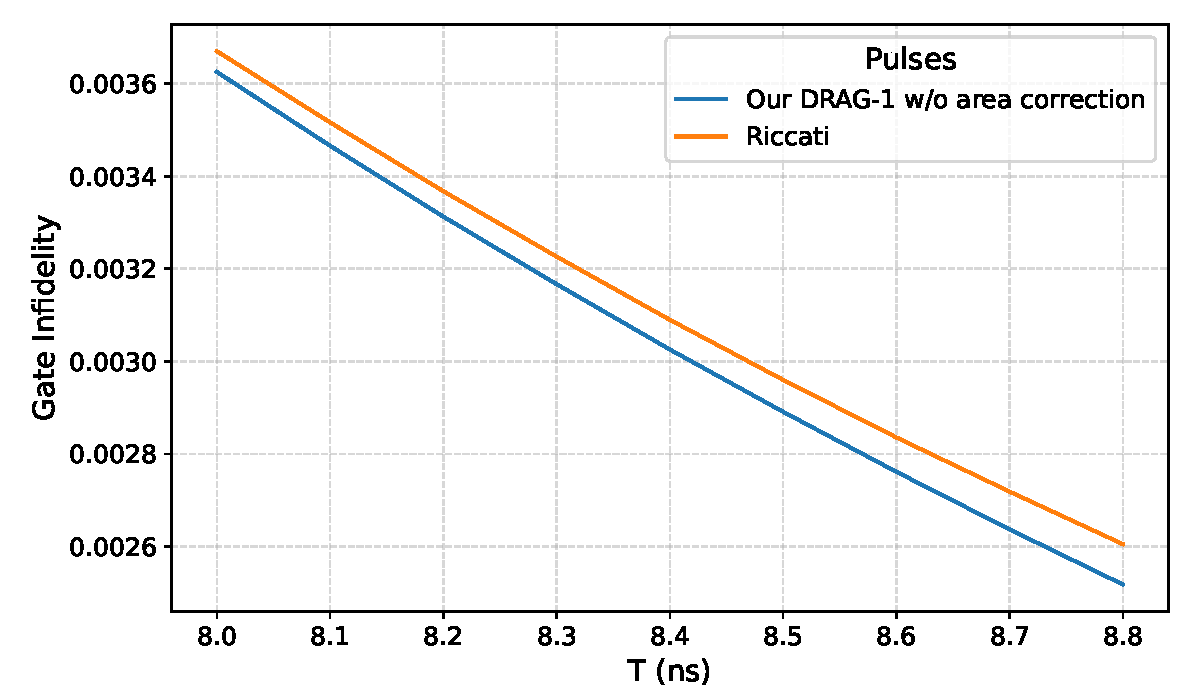
\includegraphics[width=0.8\columnwidth]{fig/fig_riccati.pdf}
  \label{fig:riccativsr1d}
  \caption{
    Our DRAG-1 pulses' performance when Riccati engineering applied.
    Riccati engineering had a little effect on gate infidelity.
  }
\end{figure}
Riccati engineering method generally failed to improve gate fidelity.
This is considered to be due to difficuly in numerical analysis.
% Further investigations
% They generally induces big error
% \subsubsection{Leakage}
% This gives us an insight that
% $\eps$

\subsection{CZ gate}
\subsubsection{Simulation}
% \epsilon
We set $N=1001$.
As in the previous research \cite{Ding2025,Martinis2014}, we simulate our designed pulses in the following fashion:
We design $\dfrac{\dd\theta}{\dd\tau}$ and then integrate to find $\theta$ in non-linear time frame.
We apply the time transformation to obtain $\theta(t)$.
We then simulate the time evolution as the two-level system described in \ref{subsec:leakage}
to find the leakage error.
We also simulate with the Hamiltonian in \eref{eq:hamiltonian_cz}
to find the phase accumulation of $\ket{00}$, $\ket{01}$ and $\ket{10}$.
We first simulate  with the normalized amplitude, changing this amplitude by an optimizer to find when the conditional
phase is close to $\pi$.
Also, Slepian pulse with $NW=2.9$ is used for reference.
% $$
%   \tilde{g}\rightarrow \tilde{\theta}\rightarrow x \rightarrow y
% $$
% Simulation conditions are
% We numerically solved the dynamics described in \ref{subsec:leakage},
% and then find $P_e$
\subsubsection{Anti-symmetric Chebyshev pulse}
\begin{figure}
  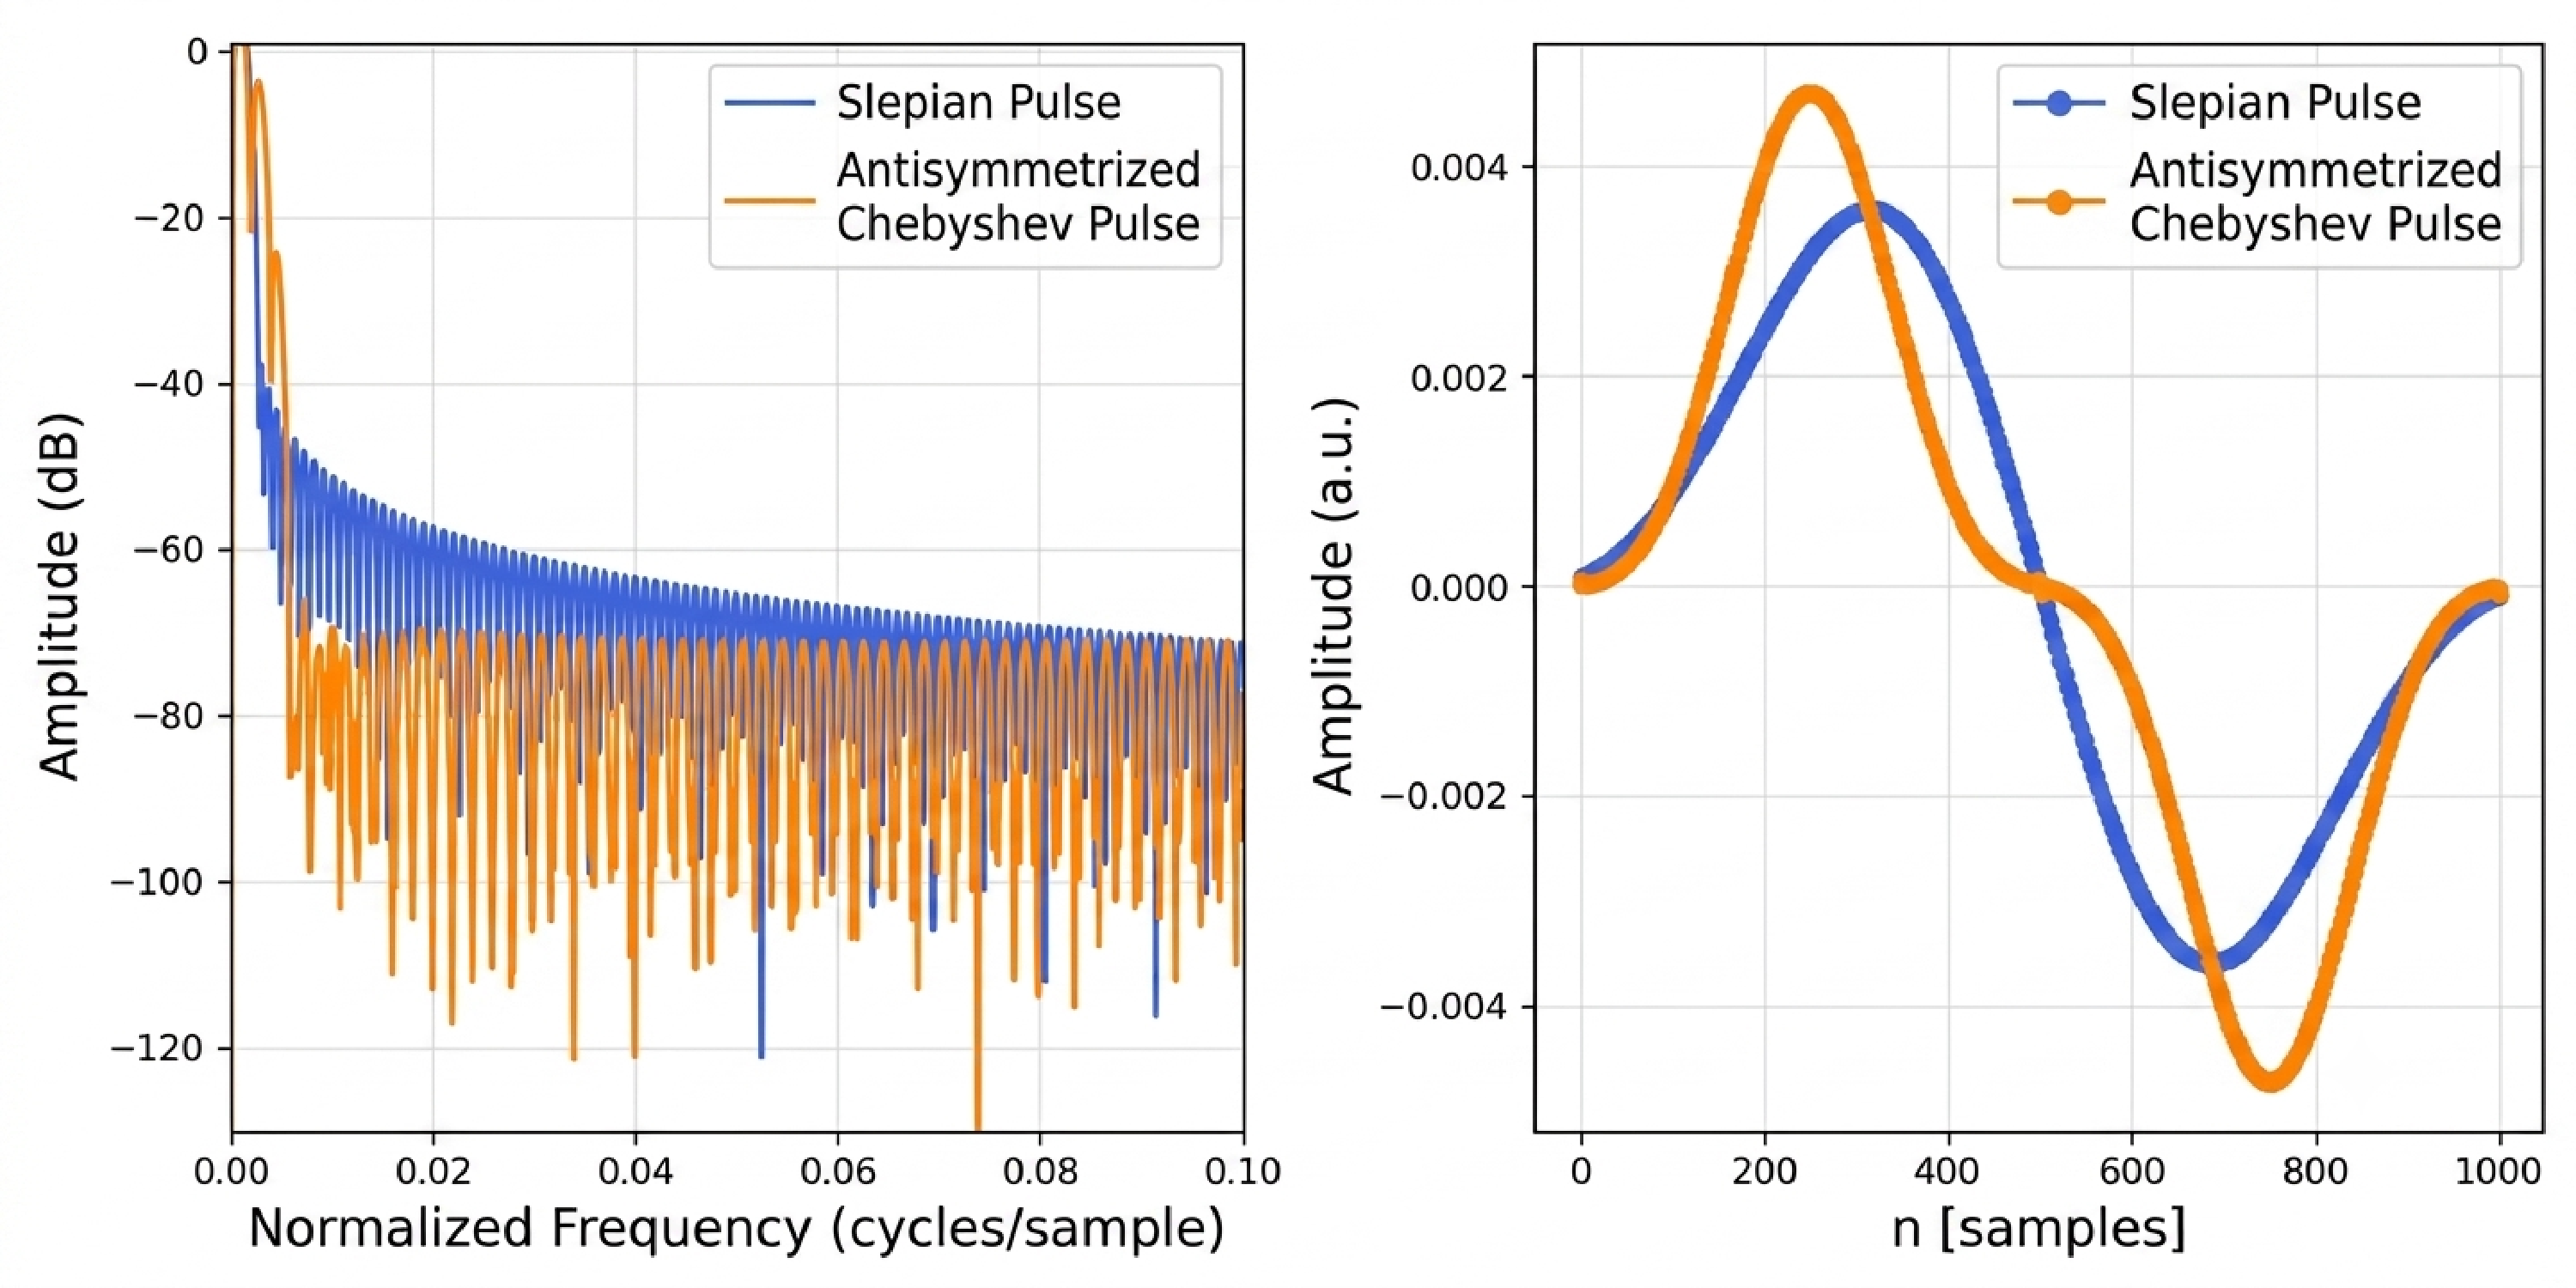
\includegraphics[scale=.3]{fig/fig_cheb_slep.pdf}
  \caption{
    The frequency domain (left) and the time domain (right) representation of Slepian and antisymmetrized Chebyshev
    pulses. The parameter $r$ is chosen so that sidelobe height is $40~\mathrm{dB}$ lower than the first slepian
    sidelobe height.
  }
  \label{fig:cheb_slep}
\end{figure}
Created with the parameter $r=0.000238$, this pulse is illustrated in \fref{fig:cheb_slep}
\subsubsection{Sidelobe-Aware Optimization}
\begin{figure}
  \centering
  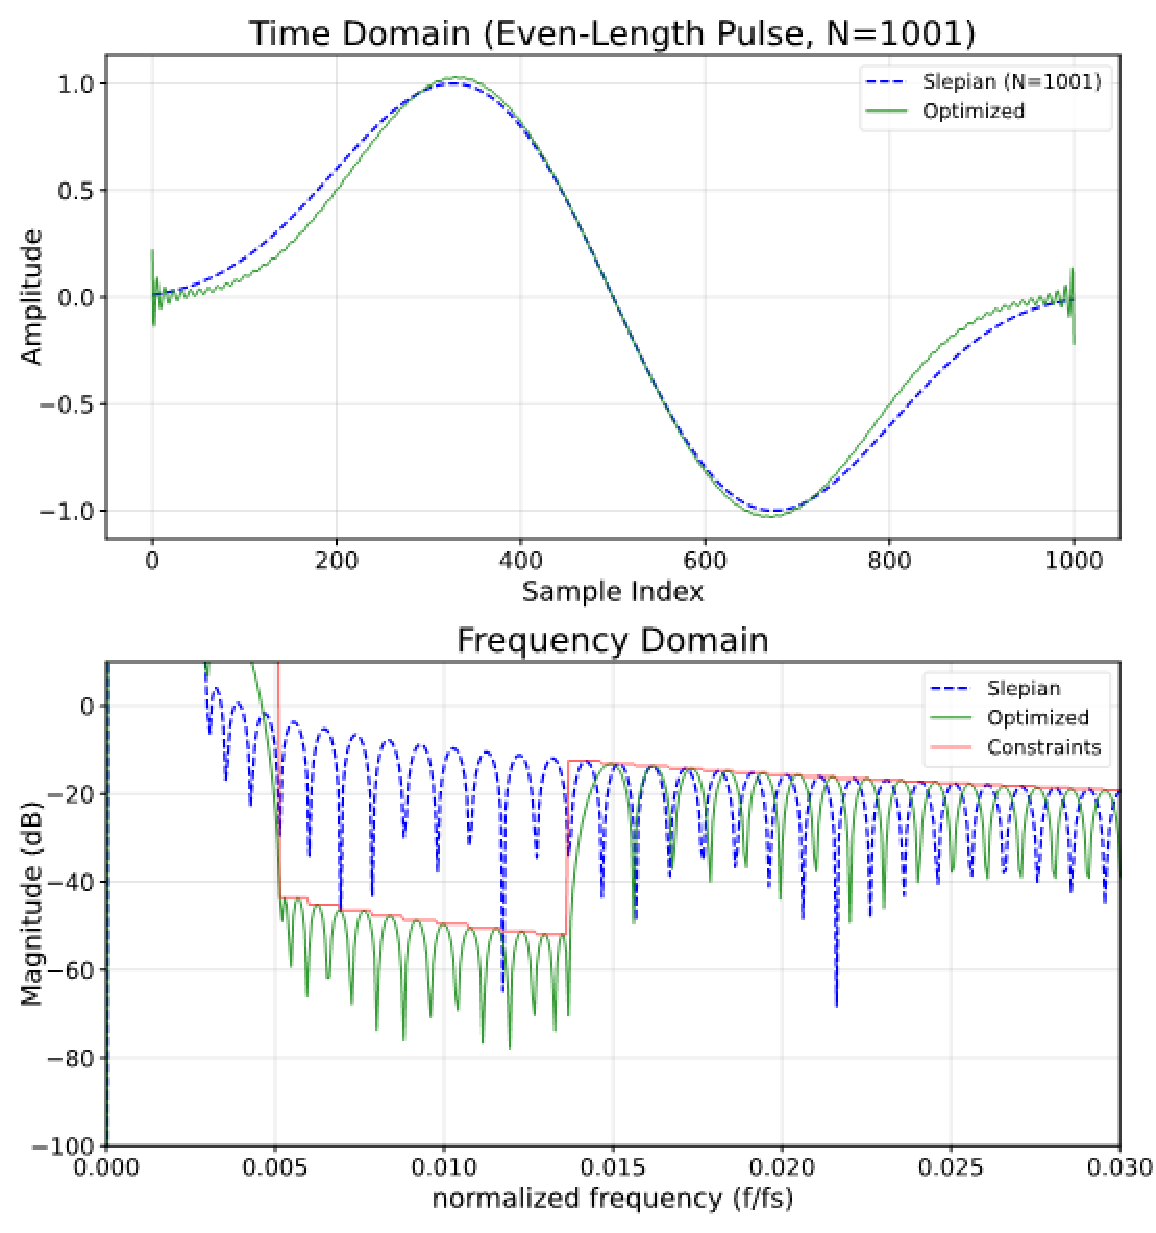
\includegraphics[scale=.5]{fig/fig_slep_opt.pdf}
  \caption{
    Slepian pulse and its optimized pulse.
    % The frequency domain (left) and the time domain (right) representation of Slepian and antisymmetrized Chebyshev
    % pulses. The parameter $r$ is chosen so that sidelobe height is $40~\mathrm{dB}$ lower than the first slepian
    % sidelobe height.
  }
  \label{fig:slep_opt}
\end{figure}
After the first four sidelobe, from $5$-th to $13$-th sidelobe heights are suppressed.
The pulse shape and its spectrum are illustrated in \fref{fig:slep_opt}.
\subsubsection{Slepian pulse with redefined maximization problem}
We set $W_1=2.9/1001$ and $W_2=8.8/1001$ to obtain a pulse with the corresponding redefined problem.
\subsubsection{Performance}
\begin{figure}[thbp]
  \centering
  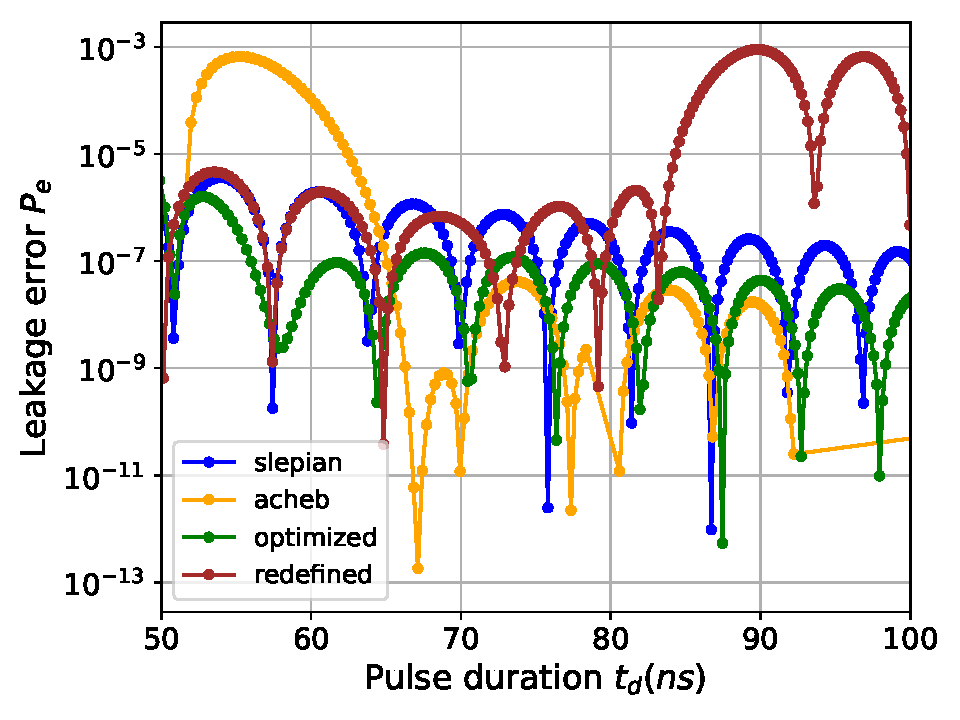
\includegraphics[width=.5\textwidth]{fig/fig_redefined.pdf}
  \caption{Leakage error of four pulses, Slepian (slepian), Anti-symmetric Chebyshev (acheb), Sidelobe-aware
    optimization (optimized), and the pulse optimized by redefining the original eigenvalue problem (redefined)}
  \label{fig:performance_cz}
\end{figure}
As illustrated in \fref{fig:performance_cz}, in overall, the optimized slepian pulse performed the best.
The anti-symmetric Chebyshev pulse performed really well at around $T=70~\text{ns}$ with suppressing leakage level by an
order of two.
The result of the Slepian pulse with the redefined problem is aligned with our expectations, larger leakage error at
unwanted gate duration times.
\subsubsection{Minimum Gate time}
\begin{figure}
  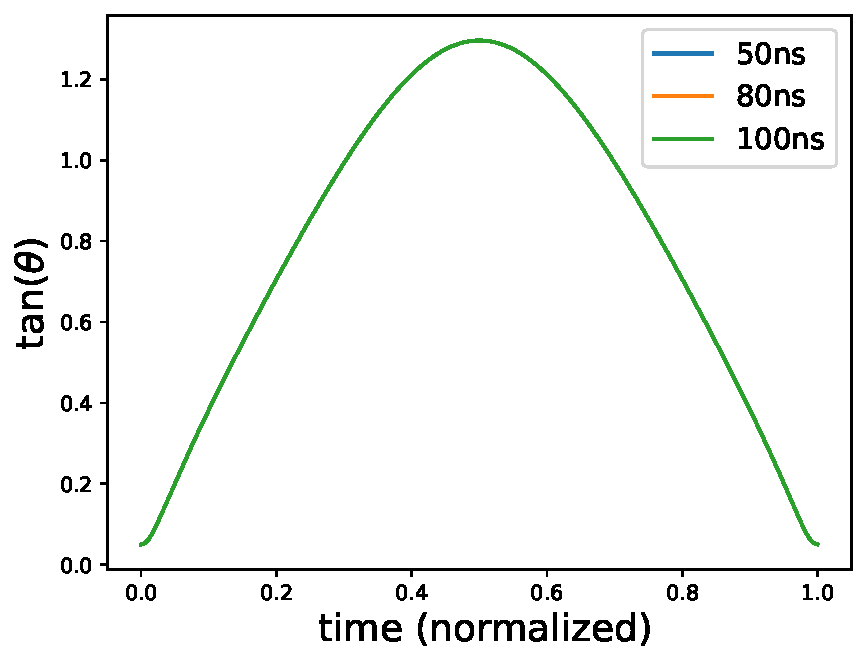
\includegraphics[scale=.5]{fig/fig_tan_5080100.pdf}
  \centering
  \caption{The relation between $T_d$ and $\tan(\theta)$ for the Slepian pulse with $T=50,80,100 $. The three
    graphs are overlapping each other due to almost the same $A(\tau_d)$.}
  \label{fig:amplitude}
\end{figure}
Once the pulse shape ${g}$ determined,
its integration ${\theta}$ is decided up to the amplitude factor $A(\tau_d)$, $(0\leq A(\tau_d)\leq1)$
$$
  {\theta} = {\theta}^n(\tau/\tau_d)A(\tau_d),
$$
where ${\theta}^n$ is the normalized ${\theta}$ that reaches $\epsilon(t_{mid})=0$ during avoided crossing.
\begin{align*}
  t(\tau) & = \int_0^\tau \sin {\theta}(\tau') \, \dd\tau'                                            \\
          & = \tau_d \int_0^{\tau/\tau_d}\,\sin \left[A(\tau_d) {\theta}^n(\tau') \right]\, \dd\tau'. \\
\end{align*}
% During this flux trajectory, the states $\vert{}00\rangle$, $\vert{}01\rangle$, and $\vert{}10\rangle$ remain largely
% isolated from any crossings. Therefore, the phases they accumulate are purely their standard, uncoupled dynamical
% phases:
% $\phi_{00} = \phi_{00}^{\text{uncoupled}}$$\phi_{01} = \phi_{01}^{\text{uncoupled}}$$\phi_{10} = \phi_{10}^{\text{uncoupled}}$
Therefore, gate duration in the lab frame is $t_d = \tau_d \int_0^1 \sin \left[A(\tau_d) {\theta}^n(\tau') \right]\, \dd\tau'$.
$t_d$ is decided upon the amplitude $A(\tau_d)$ and the initial pulse shape.
As you see in \fref{fig:amplitude},  $A(\tau_d)$ does not change over different $\tau_d$.
Hence the gate durations in $t$ and $\tau$ are proportionate.

% There are two types of phases: Berry phases and dynamical phases.
% Since the trajectory that the instantaneous $\ket{11}$ traces through the operation is a 1D path,
% thus enclosing zero area, it produces zero Berry phase.
% In formula,
% \begin{equation}
%   \phi = \int \Delta E \,\dd t = -\int \frac{\Delta}{2} \tan \frac{\theta(t)}{2} \, \dd t
% \end{equation}
%
% Since $\tan(\theta/2) = \dfrac{\tan(\theta)}{1+\sqrt{1+\tan(\theta)^2}}$
%
% % As you see in the graph of $\epsilon(t)$
% Since $0\leq\tan\dfrac{\theta(t)}{2}\leq 1$, the gate duration $T$ satisfies $T\geq \dfrac{2\pi}{\Delta}.$

% is connected through
%
% Required slew rate of DAC is


% \subsubsection{Combination of two pulses}
% Interestingly enough, their arguments are almost equal defying the possibility of mixing them together to gain a pulse
% with lower leakage.
% \subsubsection{Robustness against gate time}
% The reason behind the fact that the Slepian pulse has been used for so long days is its robustness against gate
% duration.
   % Methodology
\section{Conclusion}
Riccati engineering is applied to optimize an existing pulse,
if we could simplify the Hamiltonian somehow, could be available.
   % Methodology
\acknowledgments
I would like to express my gratitude to Professor Takashi Sato for introducing me to the realm of quantum
information and quantum control, and for providing the opportunity to undertake this research.

My deep thanks also go to Professor Kiichi Niitsu, Professor Masanori Hashimoto, Associate Professor
Rei Ueno, Assistant Professor Kotaro Matsuoka, and Professor Hiromitsu Awano (Nagoya University) for their valuable
support through research workshops and seminars.

I am uniquely indebted to Ms. Shuko Nishiyama of the Sato Laboratory support staff for her
continuous support of my day-to-day research activities. Finally, I extend my  sincere appreciation to all members of
the Integrated Systems Engineering Laboratory for creating such a vibrant and motivating research atmosphere.

Additionally, all numerical calculations and open quantum system simulations in this study were performed using the
QuTiP 5 software library in Python. The author also thanks Wolfram Research, Inc. for the use of Mathematica (Version
14.3.0) in conducting the analytical calculations.
   % Methodology

% 文献リストの出力設定
\bibliographystyle{kuissort}
\bibliography{references}

\appendix
\section{SWTs to Derive DRAG-2 Formula}
\label{appendix:DRAG2}
We successively apply the following SWTs:
\begin{align*}
  \hat{S}_4(t) & = -i\lambda_2\lambda_3\frac{\Omega_V^2(\Delta_3 -
  2\Delta_2)}{8\Delta_3\Delta_2^2}\hat{\sigma}_{1,3}^y,            \\
  \hat{S}_5(t) & =
  i\lambda_2\lambda_3\frac{(\dot{\Omega}_V\Omega_V)(\Delta_3 -
  2\Delta_2)}{(8\Delta_3^2\Delta_2^2)}\hat{\sigma}_{1,3}^x,        \\
  \hat{S}_6(t) & =
  -i\lambda_2\lambda_3\frac{\Omega_2^2(2\Delta_2 - \Delta_3)(\Delta_3^2 -
  \Delta_2^2)}{(8\Delta_2^4\Delta_3)}\hat{\sigma}_{1,3}^y          \\
  \hat{S}_7(t) & =
  i\lambda_2\lambda_3\frac{\dot{\Omega}_2\Omega_2(2\Delta_2 - \Delta_3)(\Delta_3^2 -
    \Delta_2^2)}{(4\Delta_2^4\Delta_3^2)}\hat{\sigma}_{1,3}^x.
\end{align*}

\section{Wolfram Code for Validating $Y$ DRAG Correction without Perturbation}
\begin{lstlisting}
ClearAll["Global`*"];
M = 3;
dim = M + 1;

ketbra[m_, n_] := Normal@SparseArray[{{m + 1, n + 1} -> 1}, {dim, dim}]

(* Define the Pauli operators acting on adjacent levels |j-1> and |j> *)
sigX[j_] := ketbra[j - 1, j] + ketbra[j, j - 1]
sigY[j_] := -I * ketbra[j - 1, j] + I * ketbra[j, j - 1]
sigZ[j_] := ketbra[j - 1, j - 1] - ketbra[j, j]
comm[A_, B_] := A . B - B . A

(* ==========================================
   Define the Original Hamiltonian & Generator
   ========================================== *)
H0 = Sum[(Delta[j] + j * delta[t]) * ketbra[j, j], {j, 1, M}];

Vx=Sum[lambda[j] * Omegax[t] / 2 * sigX[j], {j, 1, M}];
Vy=Sum[lambda[j] * Omegay[t] / 2 * sigY[j], {j, 1, M}];
Horig = H0 + Vx + Vy;


(* ==========================================
    Compute the Transformation
   ========================================== *)

U = Cos[-lambda[2] * Omegax[t] / (2*Delta)] * (ketbra[1,1]+ketbra[2,2]) + I * sigY[2] * Sin[-lambda[2] * Omegax[t] / (2*Delta)];
U = U + ketbra[0,0];
Hpr = U . Horig .  ConjugateTranspose[U] + I * D[U,t] . ConjugateTranspose[U];
(U . Horig .  ConjugateTranspose[U])[[1,2]];
MatrixForm[Map[Simplify, Hpr[[2,3]], {2}]];

\end{lstlisting}

% \section{逐次二次計画法 (SQP) の基礎}
\label{app:sqp}

逐次二次計画法（Sequential Quadratic Programming: SQP）は、非線形な目的関数と制約条件を持つ最適化問題を解くための強力かつ標準的な反復解法の一つである \cite{nocedal2006numerical}。本付録では、SQPアルゴリズムの基本原理と理論的背景について概説する。

\subsection{問題の定式化}
以下のような一般的な非線形最適化問題を考える。
\begin{align}
    \min_{x \in \mathbb{R}^n} \quad & f(x) \label{eq:sqp_obj} \\
    \text{subject to} \quad & c_i(x) = 0 \quad (i \in \mathcal{E}), \label{eq:sqp_eq} \\
    & c_i(x) \le 0 \quad (i \in \mathcal{I}), \label{eq:sqp_ineq}
\end{align}
ここで、$f: \mathbb{R}^n \to \mathbb{R}$ は目的関数、$c_i: \mathbb{R}^n \to \mathbb{R}$ は制約関数であり、$\mathcal{E}$ および $\mathcal{I}$ はそれぞれ等式制約と不等式制約のインデックス集合を表す。また、これらの関数は十分に滑らかである（二階連続微分可能）と仮定する。

この問題に対するラグランジュ関数（Lagrangian）$L(x, \lambda)$ は、次のように定義される。
\begin{equation}
    L(x, \lambda) = f(x) - \sum_{i \in \mathcal{E} \cup \mathcal{I}} \lambda_i c_i(x)
\end{equation}
ここで、$\lambda = (\lambda_i)_{i \in \mathcal{E} \cup \mathcal{I}}$ はラグランジュ乗数ベクトルである。最適解においては、カルーシュ・クーン・タッカー（KKT: Karush-Kuhn-Tucker）条件が成立することが知られている。

\subsection{二次計画部分問題の導出}
SQPは、ニュートン法を最適化問題のKKT条件に適用した手法と解釈できる。現在の反復点 $x_k$ において、探索方向 $d$ を求めるために、目的関数を二階テイラー展開により二次関数として近似し、制約条件を一階テイラー展開により線形近似する。これにより、次の二次計画（QP: Quadratic Programming）部分問題が得られる \cite{powell1978fast}。

\begin{align}
    \min_{d \in \mathbb{R}^n} \quad & \nabla f(x_k)^\top d + \frac{1}{2} d^\top \nabla_{xx}^2 L(x_k, \lambda_k) d \label{eq:qp_obj} \\
    \text{subject to} \quad & c_i(x_k) + \nabla c_i(x_k)^\top d = 0 \quad (i \in \mathcal{E}), \label{eq:qp_eq} \\
    & c_i(x_k) + \nabla c_i(x_k)^\top d \le 0 \quad (i \in \mathcal{I}) \label{eq:qp_ineq}
\end{align}

ここで、$\nabla_{xx}^2 L(x_k, \lambda_k)$ はラグランジュ関数のヘッセ行列（Hessian）である。

\subsection{アルゴリズムの概要}
各反復においてQP部分問題 \eqref{eq:qp_obj}--\eqref{eq:qp_ineq} を解くことで、探索方向 $d_k$ および新しいラグランジュ乗数 $\lambda_{k+1}$ が得られる。これを用いて、次のように変数を更新する。
\begin{equation}
    x_{k+1} = x_k + \alpha_k d_k
\end{equation}
ここで、$\alpha_k \in (0, 1]$ はステップ長であり、メリット関数（Merit function）を用いた直線探索（Line search）により、大域的収束性を保証するように決定される。

なお、実際の計算においては、ヘッセ行列 $\nabla_{xx}^2 L(x_k, \lambda_k)$ の厳密な計算が困難な場合が多い。そのため、準ニュートン法（例えばBFGS更新公式など）を用いて、ヘッセ行列の近似行列 $B_k$ を逐次更新する手法が一般的に用いられる。


\end{document}
